\documentclass[11pt]{article}
\usepackage{amsmath, amssymb, amsthm} 
\usepackage[spaces, hyphens]{url}
\usepackage{hyperref}
\usepackage{booktabs}
\usepackage{multirow}
\usepackage{graphicx}
\usepackage{float}

\usepackage[letterpaper, top=1in, bottom=1in, left=1.2in, right=1.2in, heightrounded]{geometry}

\setlength{\parindent}{0pt}
\setlength{\parskip}{0.6em}

\title{Evaluating Randomised Algorithms and Their LLM Generated Equivalents on the Bin Packing Problem}
\author{Joshua Raybould}
\date{March 2026}

\begin{document}

\maketitle

\section{Introduction}

\subsection{Problem Background}
The bin packing problem (BPP) is one of the central problems in combinatorial optimisation. In its standard formulation, a set of items with corresponding values (generally size or weight) must be packed into an unlimited supply of bins, each with a uniform capacity. The objective is to assign the items to the bins such that the total number of bins used is minimised. This is the one-dimensional (1D) bin packing problem, which is conceptually similar to the 1D cutting stock problem (\cite{maxence}). The 1D BPP is primarily studied in two variants: the offline problem, where the algorithm has access to the sizes of all items simultaneously, and the online problem, where items are revealed and packed one at a time. In this study, we focus on the offline case.

The 1D BPP is classified as NP-Hard, meaning that computing an exact solution requires exponential time in the worst case. Consequently, heuristic and randomised algorithms are often employed to obtain near-optimal solutions efficiently. Beyond its theoretical significance, bin packing has numerous real-world applications, ranging from loading transport vehicles with weight capacities to minimising waste in industrial cutting processes (\cite{munien}). Additionally, many complex scheduling problems contain the BPP as a special case.

\subsection{Problem Definition}
Here we formalise the classical offline 1D BPP. The following definition is relatively standard and is arrived at with reference to \cite{munien}, though equivalent normalised versions are also common in the literature (see \cite{maxence}). 

Let $C$ denote the uniform capacity of each bin, and let $s_{i}$ denote the weight or size of item $i$, such that $s_{i} \leq C$ for all items. We define $u$ as an upper bound on the minimum number of bins required to pack all $n$ items. We introduce the binary decision variable $y_{j}$, where $y_j = 1$ if the $j$-th bin is opened (used in the solution), and $0$ otherwise, for $1 \leq j \leq u$. Items are labeled $i \in \{1, \dots, n\}$, and we define a second binary variable $x_{ij}$, which equals $1$ if item $i$ is packed in bin $j$, and $0$ otherwise. The objective function is:
$$ \min\sum_{j=1}^{u} y_j $$ 
This aims to minimise the total number of open bins, subject to the following constraints:
$$ \sum_{j=1}^{u} x_{ij} = 1, \quad \forall i = 1, \dots, n $$
$$ \sum_{i=1}^{n} x_{ij} s_{i}  \leq C y_j, \quad \forall j = 1, \dots, u $$
The first constraint ensures that each item is packed into exactly one bin. The second constraint guarantees that the sum of the weights of the items in any given bin does not exceed the bin capacity $C$, and forces $y_j$ to be $1$ if any item is placed in bin $j$.

\subsection{Complexity Analysis}

The 1D offline BPP is strongly NP-hard, which can be established via a polynomial-time reduction from the 3-Partition problem \cite{garey}. Given an instance of 3-Partition consisting of $3m$ integers $a_1, \dots, a_{3m}$ where $B/4 < a_i < B/2$ for all $i$ and $\sum_{i=1}^{3m} a_i = mB$, we construct a BPP instance with bin capacity $B$ and items of exactly those sizes. A valid packing into $m$ bins exists if and only if a solution to 3-Partition exists. Since each $a_i > B/4$, no bin can hold more than three items, and since each $a_i < B/2$, no bin can hold fewer than two; every bin must therefore contain exactly three items summing to $B$. Because 3-Partition is strongly NP-complete \cite{garey}, BPP is strongly NP-hard. As a consequence, no polynomial-time algorithm for solving the BPP to optimality is known, assuming P $\neq$ NP. For large-scale instances, approximation algorithms and stochastic metaheuristics that trade guaranteed optimality for computational efficiency are therefore necessary.

\subsection{Randomised Algorithms}
Randomised algorithms rely on random variable generation to influence their execution paths, making them non-deterministic. In this context, we define stochastic optimisation as the use of randomness to navigate a search space and find near-optimal solutions efficiently (\cite{sean}). While strict definitions of stochastic optimisation often require a noisy objective function, the algorithms implemented here primarily use random choices to direct the search process. Therefore, these algorithms largely belong to the subfield of metaheuristics, which are problem-independent frameworks that guide and modify underlying heuristics to escape local optima (\cite{yang}). 

These algorithms vary drastically in complexity. The simplest approaches might involve randomising the input order before applying a naive greedy heuristic, which is particularly useful for mitigating worst-case inputs generated by adversaries. Conversely, more complex metaheuristics draw inspiration from biological evolution and natural systems. A primary goal of this paper is to benchmark a diverse variety of these approaches.

\subsection{Large Language Models (LLMs)}
LLMs are trained on massive corpora of text and code, enabling them to capture semantic meaning and structural syntax across both natural and programming languages. This has made them highly capable of generating code, as programming languages share structural similarities with natural text.

Naturally, there are limitations. The code produced by LLMs is not guaranteed to be correct and requires rigorous verification. While models perform exceptionally well on tasks heavily represented in their training data, they often lack the capacity for deep reasoning in novel scenarios \cite{kucharavy}. Consequently, for common tasks (e.g., the Mostly Basic Python Programming dataset), modern LLMs generate reliable solutions. Furthermore, while metaheuristics for the BPP are not an entirely niche domain, the empirical nature of algorithm design poses unique challenges.Specifically, selecting optimal hyper-parameters---such as cooling schedules in SimulatedAnnealing---and managing the complex interplay between different algorithmic components typically require extensive trial-and-error and human intuition. As these nuances are likely difficult to deduce from the static code found in training corpora, it remains an open question how capable LLMs are at producing performant metaheuristics.

\subsection{Research Questions}
This project aims to compare the empirical performance of human-written randomised algorithms for the 1D offline BPP against implementations generated by state-of-the-art LLMs. Specifically, our key research questions are: 
\begin{enumerate}
    \item How do various human-implemented randomised algorithms for the BPP compare in empirical performance across diverse problem instances? This establishes a robust baseline and provides insight into practical algorithmic efficiency.
    \item How effective are flagship LLMs at producing functionally correct and highly performant code for complex combinatorial optimisation problems?
    \item To what degree does performance vary across different LLMs, and are there identifiable patterns or common algorithmic shortcomings in their generated code?
\end{enumerate}

\section{Literature Review}

\subsection{Traditional Algorithms for the 1D BPP}
The 1D BPP has been extensively researched, with a vast array of exact, heuristic, and metaheuristic algorithms applied to it over the decades (TODO: cite some early papers). While numerous studies compare a small subset of these algorithms (TODO: cite some), there remains a distinct lack of comprehensive, cross-paradigm comparisons. Furthermore, the broader surveys that do exist rarely include empirical results, making it difficult to gauge how effective a specific implementation might be in practice. Because the primary goal of existing literature is often to propose novel algorithms or summarize the state-of-the-art, researchers less familiar with stochastic optimization lack a unified baseline. By evaluating both standard algorithms and recent advancements on identical problem instances, this study establishes a strong empirical foundation for evaluating BPP solvers.

\subsection{Large Language Models in Code Generation}
While LLMs were initially developed for natural language processing \cite{chang}, recent research demonstrates their emerging capability to comprehend and synthesize programming languages. Notably, experiments with models such as GPT-4 have shown that LLMs can successfully write greedy algorithms and solve dynamic programming problems, occasionally surpassing capable university students in these domains \cite{bubeck, chang}.

\subsection{Evaluating LLM Performance on Complex Tasks}
To quantify these generative capabilities, multiple studies have compared human-written code to LLM-generated solutions for competitive programming challenges, such as those found on LeetCode (\cite{bubeck}, \cite{wang}, \cite{coignion}). These problems exhibit higher logical complexity than those in standard evaluation datasets like HumanEval or Mostly Basic Python Programming (MBPP), providing a closer proxy to the difficulty of implementing BPP metaheuristics.

The findings from \cite{coignion} highlight a compelling divergence between execution efficiency and functional robustness. In terms of solution speed, LLMs frequently outperformed human developers, beating 73\% of previous submissions on average. Functional validity was also reasonable for well-known problems, averaging approximately 38\% on the most popular LeetCode questions. However, LLM performance proved highly sensitive to the novelty of the task. When evaluated on a dataset of newly released LeetCode questions, which were absent from the models' training corpora, correctness deteriorated, with the best model scoring only 9.5\% on a single-attempt basis. 

The rapid adoption of LLMs has spurred a wide range of research into their output quality, with numerous studies investigating broader software engineering concerns such as the maintainability and security of AI-generated code (TODO: cite some). However, within the context of combinatorial optimization, the primary concern remains algorithmic efficacy. Given the stark drop in correctness on novel tasks observed in competitive programming, applying LLMs to the empirical domain of BPP metaheuristics provides a rigorous test of their ability to generate performant optimization algorithms.

\section{Human-Implemented Metaheuristics}

To establish a robust empirical baseline, we implemented a diverse suite of stochastic algorithms for the 1D BPP. Parameter values were chosen based on the average percentage over the lower bound (see below), subject to a maximum average execution time of 20 seconds per run on a set of uniform instances we generated (test-u). This limit was chosen to ensure that the total runtime across 5 independent runs remained under 100 seconds, keeping algorithms with steep runtime scaling tractable at the larger instance sizes evaluated in Section 4, where no time limits are imposed.

\subsection{Common Algorithmic Components}

\subsubsection{Lower Bounds}

We first establish the theoretical lower bounds utilized as a strict stopping criterion for the evaluated algorithms. Employing a tight lower bound ensures that algorithms do not waste computational time searching once an optimal solution has been achieved. A simple, well-known lower bound on the number of bins, computable in $O(n)$ time, is given by (\cite{martello}):

\[
L_1 = \left\lceil \frac{\sum_{i=1}^{n} s_i}{C} \right\rceil
\]

This bound is derived by considering an LP-relaxation of the problem, wherein items are allowed to be fractionally split across bins. In the optimal solution for this relaxation, every open bin is filled entirely to capacity, except potentially the last, which contains the residual weight \cite{fekete}. Despite its simplicity, $L_1$ is highly effective when item weights are small relative to the capacity, guaranteeing a worst-case bound of $\frac{1}{2}$ the optimal solution value (\cite{martello}, \cite{fekete}). However, because the problem instances evaluated in this study feature larger item weights, $L_1$ is often too loose to trigger early termination.

We instead employ the $L_2$ bound developed by Martello and Toth \cite{martello}, which guarantees at worst $\frac{2}{3}$ of the optimal solution value. It requires $O(n \log n)$ time, which is dominated by the initial need to sort the items by decreasing weight. We briefly outline the bound here; for a comprehensive derivation, we direct the reader to \cite{martello}. For any integer $K$ such that $0 \le K \le \frac{1}{2} C$, the items are partitioned into three sets:

\[
\begin{aligned}
I_1 &= \left\{\, i \in \{1,\dots,n\} \;\middle|\; s_i > C - K \,\right\},\\
I_2 &= \left\{\, i \in \{1,\dots,n\} \;\middle|\; C - K \ge s_i > \tfrac{1}{2}C \,\right\},\\
I_3 &= \left\{\, i \in \{1,\dots,n\} \;\middle|\; \tfrac{1}{2}C \ge s_i \ge K \,\right\}.
\end{aligned}
\]

Martello and Toth then define the lower bound for a given $K$ as:

\[
L_2(K)=|I_1|+|I_2|+\max\!\left\{0,\left\lceil
\frac{\sum_{i\in I_3}s_i-\left(|I_2|C-\sum_{i\in I_2}s_i\right)}{C}
\right\rceil\right\}.
\]

This represents a valid bound for every possible value of $K$. The first two terms account for items in $I_1$ and $I_2$, which are strictly greater than half the bin capacity and therefore cannot share a bin with one another. The third term calculates the additional bins required if the total weight of the items in $I_3$ exceeds the combined residual space left in the $I_2$ bins. 

Because the tightness of the bound is dependent on $K$, the strongest lower bound is obtained by maximizing $L_2(K)$ across all valid $K$. To achieve the desired $O(n \log n)$ runtime, the item weights are first sorted in decreasing order, and $K$ is restricted to values that explicitly appear in the item weights. Furthermore, because any item in $I_1$ or $I_2$ is strictly greater than $\frac{1}{2}C$, the combined cardinality $|I_1| + |I_2|$ is invariant with respect to $K$. Our implementation precomputes this constant size once. Then, as we iterate through valid values of $K$, we dynamically update the continuous sums $\sum_{i \in I_2} s_i$ and $\sum_{i \in I_3} s_i$, incrementing the size of $|I_2|$ only as required for the third term. 

Note that while $L_2$ is the bound we use, there is a slightly tighter bounds which makes use of dual feasible functions, as developed by Fekete and Schepers \cite{fekete}.

\subsubsection{Fitness Evaluation}
If the objective function relies solely on the total number of active bins, the fitness landscape remains flat for the vast majority of algorithmic transitions, and so lacks the ability to guide the algorithm's search \cite{gga}. 

To circumvent this, we utilize the sum-of-squares objective function, a widely adopted approach originally introduced by Falkenauer for evolutionary bin packing \cite{gga} which is still used in modern implementations (\cite{sonuc}, \cite{kryz}). We define the fitness of a candidate solution as:
$$f = \sum_{j=1}^{u} \left( {\sum_{i=1}^{n} x_{ij} s_{i}} \right)^2$$
This yields a higher fitness score when items are concentrated into tightly packed bins rather than distributed evenly across multiple bins. This guides the algorithm to starve lightly packed bins until they can be emptied completely, thereby reducing the total bin count.

\subsection{Best Fit With Randomised Order}

\subsubsection{Overview}
Best Fit is a classic heuristic typically applied to the online version of the bin packing problem. While rarely used in isolation for the offline variant (where stronger alternatives exist), it serves as a good baseline for evaluating performance. The algorithm operates identically to the standard Best Fit, placing each item into the bin with the tightest available space—but randomises the order of the input items before execution. The purpose of this is to mitigate the impact of adversarial or worst-case input orderings, allowing the heuristic to generally achieve better packings \cite{rajeev}. We refer to this combined procedure as Randomised Best Fit (RBF).

\subsubsection{Implementation}
The algorithm first applies a Fisher-Yates shuffle to generate an unbiased random permutation of the input items. Following this initialisation, the standard Best Fit heuristic sequentially evaluates each item in the newly randomised array. For every item, the algorithm scans all currently open bins and places the item into the specific bin that minimizes the residual (leftover) capacity. If an item is too large to fit into any existing bin, the algorithm opens a new bin to accommodate it. This process continues until all items have been successfully packed.

\subsection{Simulated Annealing (SA)}

\subsubsection{Overview}
Simulated Annealing (SA) is a probabilistic metaheuristic closely related to hill-climbing. A standard hill-climbing algorithm iteratively generates neighboring candidate solutions and transitions to them only if they offer an improvement. SA modifies this approach by introducing a probability of transitioning to a worse solution. This mechanism provides the search trajectory with opportunities to escape local optima, significantly increasing the likelihood of converging on the global optimum. The probability of accepting a deleterious move depends on a temperature value; the higher this is the more likely the algorithm is to move to worse solutions. The temperature decays over time according to a predefined cooling schedule (\cite{sean}, \cite{gendreau}).

\subsubsection{Implementation}
The algorithm generates its initial candidate solution using the First-Fit Decreasing (FFD) heuristic, mirroring the initialization strategy utilized by Sonuç et al. (\cite{sonuc}). We evaluate the quality of candidate solutions using the sum-of-squares objective function previously defined. 

To transition to a neighboring solution, the algorithm selects two distinct bins at random. It then has an equal probability of either moving a single random item from the first bin to the second, or swapping two random items between them. Any move that would cause a bin to violate its capacity constraint is immediately rejected, leaving the candidate solution unchanged.

We initialize the temperature $T = 1{,}000{,}000$ and set a maximum number of iterations $I = 1{,}500{,}000$. We utilize an exponential (geometric) cooling schedule with $\alpha = 0.9995$, a widely adopted choice in practice \cite{gendreau}. While this $\alpha$ value is high, empirical testing revealed that lower values caused 
the search to stagnate prematurely. This is likely because the FFD initialization already provides a strong starting point, bounding the initial solution to at worst $\frac{11}{9}\text{OPT} + \frac{6}{9}$ \cite{dosa}. The algorithm terminates when either $T \le 0.01$ or $I$ iterations have occurred.

\subsection{Tabu Search (TS)}

\subsubsection{Overview}
Tabu Search (TS) is a metaheuristic designed to overcome the primary limitation of standard local search methods: getting trapped in local optima. It functions similarly to hill-climbing but incorporates a short-term memory structure known as a tabu list. This list records recently visited configurations, forbidding the algorithm from returning to them for a set number of iterations. By making recent moves tabu, the algorithm is forced to explore novel regions of the search space, allowing it to escape local optima and discover stronger global configurations \cite{sean, gendreau}.

\subsubsection{Implementation}
Similar to our Simulated Annealing approach, the TS algorithm generates an initial candidate solution using the First-Fit Decreasing (FFD) heuristic and evaluates fitness using the sum-of-squares objective function. 

During each iteration, the algorithm explores the localized neighborhood by generating 30 candidate moves. A move consists of selecting two random bins and either swapping two items between them or moving a single item from one to the other. To aggressively reduce the total bin count, we implement a targeted heuristic inspired by Lodi et al. \cite{lodi}: when moving a single item, there is a 60\% probability that the algorithm will deliberately select the least full bin as the source. Because the emptiest bins are the easiest to empty entirely, this actively guides the search toward configurations that utilize fewer bins.

The algorithm executes for $I = 21{,}500$ iterations, selecting the best valid neighbor in each step even if it results in a lower fitness score than the current state. To prevent cycling without incurring excessive computational overhead, we maintain a tabu list of length 8 that stores the specific configurations of recently altered bins rather than entire solution states. Finally, we implement a standard aspiration criterion: the tabu status of a move is completely ignored if executing that move directly results in the elimination of a bin, as this guarantees a strict improvement to the global objective.

\subsection{Variable Neighbourhood Search (VNS)}

\subsubsection{Overview}
Introduced by Mladenović and Hansen \cite{mladenovic}, VNS is a metaheuristic that works by systematically changing neighbourhoods during a perturbation phase (shaking) followed by a local search (often called the descent phase) \cite{gendreau}. 

The algorithm requires defining a set of neighbourhood structures, $N_{k}$, for $1 \le k \le k_{\max}$, where $k_{\max}$ is a user-specified parameter. A neighbourhood $N_{k}$ could, for example, be defined as being $k$ moves away from the current solution. In each iteration of the algorithm, we start with $k = 1$ and continue until $k = k_{\max}$. While $k \le k_{\max}$, we obtain a new candidate solution by "shaking" the incumbent solution, moving from the incumbent to a random solution within its $k$-th neighbourhood. We then apply a local search to this new candidate solution. This is often executed using best improvement (which takes the direction of steepest descent) or first improvement (which selects the first discovered move that improves the solution). 

After the local search, the resulting solution is evaluated using the objective function. If this new solution is strictly better than the incumbent, it becomes the new incumbent, and $k$ is reset to 1. Otherwise, $k$ is incremented to explore a wider neighbourhood. By systematically exploring larger neighbourhoods, the algorithm significantly increases its probability of escaping the current local optimum. As noted in \cite{gendreau}, local minima with respect to one or several $N_{k}$ are relatively close to one another, implying that local optima tend to contain structural information about the global optimum.

\subsubsection{Implementation}
We generate our initial incumbent solution using the FFD heuristic. It should be noted that much of our implementation is inspired by the approach of Fleszar and Hindi \cite{kryz}, who utilize a different heuristic called Minimum Bin Slack (MBS) that generally outperforms FFD \cite{gupta}. Fleszar and Hindi’s VNS algorithm improves the solution arrived at by their $\mathrm{MBS}'$ heuristic in approximately 23\% of cases. We deliberately chose to utilize FFD instead of MBS to maintain a more consistent initialization baseline across our algorithms, ensuring that any performance differences observed are attributable to the VNS mechanism rather than the starting heuristic. Additionally, FFD is more widely used. 

Following initialization, we measure solution fitness using the sum-of-squares objective function. To optimize the local search phase, we sort our items by weight in non-decreasing order. During the shaking phase, we maintain a list of items that have not yet been moved. The algorithm selects an unmoved item at random and attempts to move it (either by swapping it with another unmoved item or transferring it to a different bin, provided capacity constraints are satisfied). Once an item is involved in a move, it is removed from the eligible list for the remainder of that shaking step. 

After shaking, we execute a best-improvement local search by systematically evaluating every possible move across the entire solution space. Specifically, for each eligible item (excluding those in completely full bins), the algorithm evaluates transferring it to every other open bin, as well as swapping it with every other eligible item. The move that yields the greatest improvement is selected. To optimize execution, the $\Delta$ fitness improvement is calculated by considering only the bins where weights actually change, as the squared sum of all other bins remains constant. 

 Because the items are processed in non-decreasing order of weight, we can speed up the search. When iterating through items to transfer into a specific bin, the inner loop terminates immediately upon encountering an item whose weight exceeds the available residual space. Similarly, when iterating through potential swap candidates $j$ for a given item $i$, the inner loop breaks as soon as the weight of $j$ exceeds the combined weight of item $i$ and the residual space in $i$'s current bin.

The algorithm terminates when the theoretical lower bound is reached or after a strict limit of 15 iterations. We set $k_{\max} = 6$, as empirical testing demonstrated that this threshold provides competitive solutions without incurring the unreasonable computational costs associated with exhaustively searching larger neighbourhoods.

\subsection{Greedy Randomised Adaptive Search Procedure (GRASP)}

\subsubsection{Overview}
GRASP is a multi-start metaheuristic consisting of two main phases: a constructive phase and a local search phase \cite{gendreau}. These two phases are executed iteratively, and the highest-quality solution found across all iterations is ultimately returned. 

The construction phase generates a candidate solution by iteratively adding components. Rather than acting purely greedily, it selects components at random from a Restricted Candidate List (RCL)—a subset of the remaining components that yield the lowest cost or highest quality. The RCL is typically defined by a threshold quality. For example, if $q^{\min}$ and $q^{\max}$ denote the qualities of the worst and best available components respectively, the threshold is defined as $q^{\min} + (1 - \alpha)(q^{\max} - q^{\min})$, where $\alpha \in [0, 1]$ controls the greediness of the search. An $\alpha$ value of 0 results in a purely greedy construction, while an $\alpha$ value of 1 results in a completely random construction. 

Various enhancements can be applied to the standard GRASP framework. In Reactive GRASP, the parameter $\alpha$ is not fixed. Instead, the algorithm initializes with a discrete set of possible $\alpha$ values, each with an equal probability of selection. As the search progresses, these probabilities are periodically updated based on the historical performance of each $\alpha$ value. This feedback loop forces the algorithm to learn from previous iterations and bias the search toward parameters that yield superior solutions. Another notable enhancement is path-relinking, an intensification strategy that explores the trajectory connecting two high-quality solutions found during the search to discover potentially superior intermediate configurations.

\subsubsection{Implementation}
We implemented a Reactive GRASP metaheuristic which runs for 10 iterations. During the constructive phase, the quality of an item is defined purely by its weight (size). Items are sequentially packed into the currently open bin. A new bin is only opened if no unassigned item can fit within the residual capacity of the active bin; otherwise, the algorithm restricts its selection exclusively to items that can successfully fit. 

To govern the RCL, we define a candidate set of $\alpha$ values: $\{0.05, 0.10, 0.15\}$. These relatively small values heavily bias the construction toward pure greediness, which is highly effective given that item weight is a strong heuristic for the Bin Packing Problem (empirical testing revealed that $\alpha = 0.05$ consistently yielded the best performance). Initially, each candidate value has an equal probability of selection. We track the average cost (defined as the total number of bins used) of the solutions generated by each $\alpha$. 

Every two iterations, provided every $\alpha$ has been utilized at least once, the selection probabilities are updated. Let $\{\alpha_1, \alpha_2, \dots, \alpha_m\}$ denote the set of candidate values. The selection probability $P(i)$ for the $i$-th value, $\alpha_i$, is calculated as:
$$Q(i) = \frac{N}{\operatorname{avgcost}(i) - \ell \cdot \min_{1 \le j \le m} \operatorname{avgcost}(j)}$$
$$P(i) = \frac{Q(i)}{\sum_{j=1}^{m} Q(j)}$$
where $Q(i)$ represents the relative performance quality of $\alpha_i$, and $\operatorname{avgcost}(i)$ is the historical average cost of solutions generated using $\alpha_i$. The numerator $N$ represents the total number of items being packed, included as a scaling factor for precision. 

The parameter $\ell$ serves as a learning rate ($0 \le \ell < 1$) that dictates how aggressively the probabilities are altered. Because the absolute difference in average bin counts between $\alpha$ values is often exceedingly small, $\ell$ is necessary to mathematically amplify these fractional differences. We set $\ell = 0.995$, allowing the probabilities to evolve organically over time without permitting any single $\alpha$ value to become overwhelmingly dominant, which would prematurely stifle exploration of the search space. Following the construction of a candidate solution, we execute the descent phase. For this, we directly utilize the Tabu Search metaheuristic defined previously. To balance intensification with computational efficiency, the inner Tabu Search is given 2,125 iterations per GRASP cycle.

\subsection{Grouping Genetic Algorithm (GGA)}

\subsubsection{Overview}
The Genetic Algorithm (GA) is a population-based evolutionary metaheuristic inspired by natural selection. A standard GA maintains a population of candidate solutions (chromosomes) and iteratively applies breeding, crossover, and mutation operators to evolve the population toward an optimal solution. 

However, as famously noted by Falkenauer \cite{gga}, standard GAs perform exceptionally poorly on grouping problems like the 1D Bin Packing Problem. In a standard GA, the chromosome encodes information at the item level (e.g., which bin an item belongs to). When standard crossover operators are applied to these item-oriented strings, they completely destroy the carefully optimized structures of well-packed bins, resulting in highly unfit children. 

To resolve this, Falkenauer introduced the Grouping Genetic Algorithm (GGA). The core innovation of the GGA is a paradigm shift in the encoding scheme: rather than focusing on the items, the chromosome encodes the groups (the bins themselves). The length of the chromosome is therefore variable, equaling the number of active bins. This ensures that when crossover and mutation operators are applied, they manipulate, transfer, or delete entire, intact bins rather than scattering individual items.

\subsubsection{Implementation}
While our foundational encoding follows Falkenauer, the majority of our genetic operators and heuristics are directly based on the state-of-the-art GGA-CGT (Controlled Gene Transmission) framework proposed by Quiroz-Castellanos et al. \cite{quirozca}. We maintain a relatively small population size of 18 chromosomes over a strict limit of 110 generations, as the complex genetic operators incur a significant computational cost. Fitness is evaluated using the sum-of-squares objective function.

To initialize the population, we employ the specialized First-Fit initialization strategy detailed in the GGA-CGT framework. The algorithm first identifies all items with a weight strictly greater than half of the bin capacity. Because these items can never share a bin with one another, they are immediately placed into their own distinct bins. The remaining items are then randomized and packed using the standard First-Fit heuristic. This guarantees a strong, structurally sound starting population.

To transition between generations, we utilize a standard elitist survival strategy: the highest-fitness individuals (the elites) are preserved intact and carried directly into the next generation. The remainder of the population is completely replaced by newly generated children. 

To generate these children, we implement a parent selection mechanism inspired by the Controlled Gene Transmission (CGT) strategy \cite{quirozca}. Rather than selecting parents purely based on fitness probability or standard tournament selection, we control the mating pairs. For each required child, a parent pair is formed by drawing one parent randomly from the elite set and the second parent randomly from the non-elite set. This approach guarantees that high-quality, proven genetic material from the elites is consistently transmitted to the offspring, while the non-elite parents inject necessary structural diversity to prevent premature convergence.

Because crossover is highly disruptive and computationally expensive, it is applied to the selected parents with only a 40\% probability. Our crossover operator sorts the bins within both parents in descending order of fullness. It then iterates through the parents, comparing corresponding bins and attempting to inherit the fullest one. If inheriting a bin would introduce a duplicate item (an item already present in a previously inherited bin), that candidate bin is rejected entirely. 

Whether a child is generated via crossover or simply cloned from a parent, it is subjected to mutation. Our mutation operator deletes exactly three bins from the chromosome. One of these deleted bins is deterministically chosen as the least full bin in the solution, helping to actively guide the search toward a lower bin count, while the other two are selected at random. 

 Following both crossover and mutation, chromosomes are frequently left with unassigned (free) items. To repair these solutions, we apply the rearrangement by pairs procedure from the GGA-CGT framework \cite{quirozca}. This procedure operates in two distinct stages. First, it iterates through a randomized permutation of the active bins and attempts to improve their packing density by swapping pairs of packed items with free items. Specifically, it searches for opportunities to replace two packed items with either a single heavier free item, or a pair of free items that fills the bin more effectively without violating capacity constraints. Any packed items removed during this process are added to the pool of free items. In the second stage, all remaining free items are reinserted into the solution using the First-Fit heuristic. To encourage optimal bin filling, these items are sorted in descending order of weight if the largest free item exceeds half the bin capacity; otherwise, they are processed in a random order.

\subsection{Ant Colony Optimisation (ACO)}

\subsubsection{Overview}
Ant Colony Optimisation (ACO) is a population-based metaheuristic inspired by the foraging behaviour of real ants. While initially moving randomly, ants leave behind chemical pheromone trails. Over time, ants travelling along shorter paths return to the nest faster, causing pheromone to accumulate more rapidly on those routes. Subsequent ants probabilistically favour paths with higher pheromone concentrations, creating a positive feedback loop that eventually guides the entire colony toward the shortest path. 

First introduced as Ant System (AS), the framework has seen significant evolution through variants like Elitist AS and MAX-MIN Ant System (MMAS) \cite{stuetzle}, making it highly competitive for complex combinatorial problems \cite{levine}. 

In ACO, artificial ants iteratively construct solutions by selecting components. The probability $p_k(i,j)$ of an ant $k$ transitioning from state $i$ to component $j$ is governed by the following standard equation (\cite{aaron}, \cite{gendreau}):
$$p_k(i,j) = \begin{cases} \frac{[\tau(i,j)]^{\alpha}[\eta(i,j)]^{\beta}}{\sum_{c \in C_k(i)} [\tau(i,c)]^{\alpha} [\eta(i,c)]^{\beta}} & \text{if } j \in C_k(i), \\ 0 & \text{otherwise}. \end{cases}$$
Here, $\tau(i,j)$ represents the accumulated pheromone (the learned historical quality of the component), and $\eta(i,j)$ represents a heuristic value. The parameters $\alpha$ and $\beta$ control the relative influence of the pheromone and the heuristic, respectively. $C_k(i)$ represents the set of feasible components that ant $k$ can currently add to its solution. Once all ants have constructed complete solutions, the pheromone trails are updated: pheromone is added based on the quality of the solutions found, and a global evaporation parameter, $\rho$, is applied to progressively forget older, suboptimal paths and prevent premature convergence.

\subsubsection{Implementation}
Our implementation was heavily guided by Levine \cite{levine}. To mitigate computational overhead and maintain feasible runtimes, we utilize a highly constrained search space consisting of just 4 ants executed over 5 iterations. Through empirical testing and parameter tuning, we observed that this shortened execution window necessitated a heavier reliance on greedy choices over historical pheromone accumulation. Consequently, we set the heuristic importance quite high at $\beta = 10$, with the pheromone importance at $\alpha = 2$ and the evaporation rate at $\rho = 0.2$. The heuristic value $\eta$ for an item is defined simply as its weight. 

Rather than assigning pheromone to specific item indices, we assign pheromone between item weights. If two items of specific weights frequently appear together in high-quality bins, the pheromone value between those weights increases. To calculate the aggregate pheromone value for a candidate item $j$ being considered for an active bin $b$, we use the adaptation from Levine:
$$\tau_b(j) = \begin{cases} \frac{1}{|b|}\sum_{i \in b} \tau(i,j) & \text{if } b \neq \varnothing \\ 1 & \text{otherwise}. \end{cases}$$
This dictates that if item $j$'s weight historically pairs well with the weights already present in bin $b$, it will have a higher probability of selection. If the active bin is empty (i.e., a new bin has just been opened), the pheromone score evaluates to 1, making the initial selection heavily dependent on the heuristic $\eta$. 

When a solution is completed, the pheromone matrix is updated by first multiplying existing values by $(1 - \rho)$ to simulate evaporation. Pheromone is then deposited based on the fitness of the solution, calculated using the normalized sum-of-squares objective function established by Falkenauer \cite{gga}. The deposited amount is the product of the solution's fitness and the frequency of each weight pair within that solution.

To aggressively refine the search space, we incorporate three core concepts from the MAX-MIN Ant System (MMAS) introduced by Stützle and Hoos \cite{stuetzle}:
\begin{enumerate}
    \item Iteration-Best and Global-Best Updates: In each standard iteration, only the iteration-best ant is permitted to deposit pheromone. Furthermore, every $\gamma$ iterations, the global-best ant updates the matrix. We set $\gamma = \lceil 500/n \rceil$, a threshold designed to control the balance between exploration and exploitation within our condensed iteration limit. 
    \item Pheromone Trail Limits: To prevent stagnation, pheromone values are strictly bounded between $\tau_{\min}$ and $\tau_{\max}$. If a value drops below $\tau_{\min}$, it is reset to the boundary. Adapting from \cite{stuetzle}, we calculate these bounds as:
    $$\tau_{\max} = \frac{1}{1-\rho}$$
    $$\tau_{\min} = \frac{\tau_{\max}\left(1 - \sqrt[n]{p_{best}}\right)}{(avg - 1)\sqrt[n]{p_{best}}}$$
    where $p_{best}$ is the probability of constructing the best solution after the trails have converged, set here to 0.05, and $avg$ is $n/2$. It is worth noting this is an approximation in the context of the BPP; because the order of items placed within a bin does not alter the final configuration, the mathematical assumptions underpinning $\tau_{\min}$ are slightly skewed. Additionally, because weight pairs can appear multiple times within a single solution, $\tau_{\max}$ acts as a soft reference rather than a strict upper limit.
    \item Optimistic Initialization: To encourage broad early exploration, all initial pheromone values are optimistically set to $\tau_{\max}$.
\end{enumerate}

\subsection{Fitness Dependent Optimizer (FDO)}

\subsubsection{Overview}
Introduced in 2019 by Abdullah and Ahmed \cite{abdullah}, the Fitness Dependent Optimizer (FDO) is a population-based swarm intelligence metaheuristic. While it shares foundational mathematical similarities with Particle Swarm Optimization (PSO)—specifically the concept of updating a search agent's position by adding a velocity or "pace" vector—FDO calculates this pace entirely differently. 

 Biologically, FDO is inspired by the reproductive swarming process of honey bees, specifically the behaviour of scout bees searching for a new hive. When a colony swarms, scout bees explore the environment to identify suitable targets. Once high-quality candidate hives are found, the scouts communicate this information to the swarm. When a consensus threshold is reached, the entire swarm navigates toward the best-identified location. 

In the context of FDO, candidate solutions represent the scout bees, and the globally optimal solution represents the target hive. The algorithm initializes a population of scout bees that randomly explore the search space. During each iteration $t$, the position of a search agent $X_i$ is updated according to the rule:
$$X_{i, t+1} = X_{i, t} + pace$$
The $pace$ variable dictates the direction and magnitude of the agent's movement and is governed by a fitness weight factor, $fw$. For maximization problems, this is specifically defined as \cite{awlla}:
$$fw = \left| \frac{f(X_{i,t})}{f(X^*)} \right| - wf$$
where $f(X_{i,t})$ is the fitness of the current agent, $f(X^*)$ is the fitness of the global best solution discovered so far, and $wf \in [0, 1]$ is a user-defined weight factor that explicitly controls the convergence rate. A $wf$ value closer to 1 generally forces rapid convergence and exploitation, whereas a value closer to 0 promotes stability and broader exploration.

\subsubsection{Implementation}
Our implementation adapts the FDO framework for the discrete 1D Bin Packing Problem, drawing heavily upon the combinatorial translation proposed by Abdul-Minaam et al. \cite{abdulminaam}. 

We initialize a population of 10 candidate solutions using the First-Fit heuristic. To optimize computational efficiency during the search phase, we maintain a direct mapping of each item to its current bin assignment, eliminating the need to exhaustively search the solution structure when validating candidate moves. Fitness is evaluated using the sum-of-squares objective function. We maintain a strict execution limit of 150 iterations, terminating early only if the theoretical lower bound is achieved.

At the beginning of each iteration, we identify both the global best solution ($X^*$) and the worst solution in the current active population. To introduce a strong elitist pressure and accelerate convergence, the worst solution in the population is immediately overwritten by a copy of $X^*$, ensuring the swarm's search is heavily anchored around the most promising known region \cite{abdulminaam}. 

Because BPP is a combinatorial problem, "adding pace" cannot be achieved via standard vector addition. Instead, $pace$ is defined as a discrete sequence of valid item transfers, defined by the tuple (item, current bin, target bin). For each solution, we calculate $fw$ using the standard FDO equation. Empirical testing demonstrated that $wf > 0$ severely degraded solution quality for our specific objective function, so we strictly set $wf = 0$. Consequently, $fw$ simplifies to the pure fitness ratio between the current solution and the global best. 

The composition of the $pace$ sequence is determined by a branching logic based on $fw$:
\begin{enumerate}
    \item Random Exploration ($fw = 0$ or $fw = 1$): The algorithm generates a random threshold $r \in [0,1]$. A proportion of the total items equal to $r$ is randomly selected. For each selected item, the algorithm attempts to transfer it to a randomly selected target bin. 
    \item Directed Exploitation ($fw \notin \{0, 1\}$): The calculated $fw$ ratio itself is used as the threshold proportion. The algorithm selects a proportion of items equal to $fw$. However, instead of moving them randomly, each selected item is aggressively directed toward the specific bin it currently occupies within the global best solution ($X^*$).
\end{enumerate}

During the construction of the $pace$ sequence, every proposed transfer is evaluated against the capacity constraints of the target bin. Invalid moves are rejected. Once the sequence is finalized, the moves are executed, the solution's fitness is recalculated, and any resultant empty bins are purged from the chromosome.

\section{Experimental Setup and Methodology}

\subsection{Instance Generation}
To evaluate the scaling behavior, computational efficiency, and solution quality of our implemented metaheuristics, we generated our own custom datasets. The generation methodology was inspired by the randomly generated classes established by Delorme, Iori, and Martello \cite{BPPLIB}. 

We generated instance sets of sizes $n \in \{100, 200, 400, 600, 800, 1000, 1200, 1400, 1600\}$ to observe performance trajectories from small-scale to large-scale problems. For each instance, the item weights were generated dynamically to ensure combinatorial complexity. For example, to prevent the generation of excessively large items that cannot be paired (which trivializes the packing process), we bounded the possible item weights relative to the bin capacity $C$. 

For each instance, a minimum weight threshold was uniformly sampled between 10\% and 30\% of $C$, and a maximum weight threshold was uniformly sampled between 50\% and 70\% of $C$. The actual item weights were then generated by sampling from a uniform distribution bounded by these instance-specific thresholds. The resulting floating-point values were rounded to the nearest integer and sorted. 

Because the true optimal configurations for these custom instances are unknown, we evaluate the absolute solution quality of our algorithms against the same lower bound ($L_2$) used by each algorithm.

\subsection{Execution Environment}
The algorithms were implemented in Python 3.11.2, utilizing native data structures (such as lists and dictionaries) to handle bin creation, item swapping, and structural mutation inherent to the metaheuristics. All computational experiments were conducted on a machine equipped with an AMD Ryzen 7 5825U CPU (1.6GHz base, 4.5GHz boost), 16GB of RAM, running Debian GNU/Linux 12 (Bookworm).

\subsection{Evaluation Metrics and Testing Procedure}
Because the implemented metaheuristics rely on stochastic processes (such as random initializations, probabilistic selections, and randomized neighborhood explorations), their performance can naturally fluctuate between executions. Evaluating a stochastic algorithm based on a single run per instance provides an unreliable, high-variance snapshot of its capability. To ensure statistical reliability and capture the true average-case behavior, every algorithm was executed 5 independent times for each generated problem instance. 

We evaluate and compare the performance of the algorithms using two primary metrics, denoted in our upcoming results tables as Execution Time (s) and Percentage Difference (dif\%).

\begin{enumerate}
    \item Execution Time (s):\\
    The computational time required by the algorithm to generate a solution. For a given problem instance, we record the physical time taken in seconds for each of the 5 independent runs and calculate the mean execution time. This provides an empirical measure of the algorithm's operational efficiency and computational scaling behavior as the instance size increases.

    \item Percentage Difference (dif\%):\\
    This quantifies the algorithm's relative, average-case solution quality compared to the theoretical lower bound. For a given instance $i$, let $R = 5$ be the total number of independent runs, and let $S_{i,r}$ be the total number of bins utilized by the algorithm during run $r$. 

    First, we calculate the average number of bins used by the algorithm across all runs for that specific instance:
    $$\bar{S}_i = \frac{1}{R} \sum_{r=1}^{R} S_{i,r}$$

    Next, we calculate the specific difference for instance $i$ as the ratio of this average to the theoretical lower bound $L_{2,i}$, minus one:
    $$Dif_i = \left( \frac{\bar{S}_i}{L_{2,i}} \right) - 1$$

    Finally, to evaluate how an algorithm scales across different problem sizes, these individual differences are averaged across all instances within a specific size class (e.g., all instances where $n=100$). This aggregated percentage difference provides a robust, standardized measure of how closely the algorithm consistently approximates the optimal solution, effectively neutralizing the variance introduced by the stochastic metaheuristic elements.
\end{enumerate}

\section{Evaluation of Human-Crafted Metaheuristics}

To establish the relative capabilities of the human-crafted metaheuristics, all eight 
implementations were evaluated across the generated custom datasets. These results 
characterise each algorithm's baseline performance and serve as the human reference point 
for the LLM comparison conducted in Section~\ref{sec:llm-eval}.

Table~\ref{tab:mega_baseline} details the average execution time in seconds and the percentage difference (dif\%) from the theoretical lower bound for each algorithm as the instance size ($n$) scales from 100 to 1600 items. The algorithms are ordered from left to right by overall average solution quality.

\begin{table}[H]
\centering
\caption{Performance Metrics of Human-Crafted Metaheuristics: Execution Time (s) and Percentage Difference (dif\%) ordered by overall average solution quality.}
\label{tab:mega_baseline}
\resizebox{\textwidth}{!}{
\begin{tabular}{l cc cc cc cc cc cc cc cc}
\toprule
\multirow{2}{*}{$n$} & \multicolumn{2}{c}{GGA} & \multicolumn{2}{c}{SA} & \multicolumn{2}{c}{TS} & \multicolumn{2}{c}{GRASP} & \multicolumn{2}{c}{VNS} & \multicolumn{2}{c}{ACO} & \multicolumn{2}{c}{FDO} & \multicolumn{2}{c}{RBF} \\
\cmidrule(lr){2-3} \cmidrule(lr){4-5} \cmidrule(lr){6-7} \cmidrule(lr){8-9} \cmidrule(lr){10-11} \cmidrule(lr){12-13} \cmidrule(lr){14-15} \cmidrule(lr){16-17}
 & Time & dif \% & Time & dif \% & Time & dif \% & Time & dif \% & Time & dif \% & Time & dif \% & Time & dif \% & Time & dif \% \\
\midrule
100  & 1.60   & 1.09 & 8.60   & 0.90 & 13.73 & 2.40 & 13.32 & 2.34 & 0.68   & 3.11 & 0.52   & 3.31 & 1.31   & 5.02 & 0.01 & 8.11 \\
200  & 4.17   & 1.03 & 12.51  & 0.79 & 17.44 & 2.27 & 17.11 & 2.44 & 2.10   & 2.95 & 1.96   & 3.33 & 3.23   & 5.51 & 0.02 & 7.45 \\
400  & 11.30  & 2.10 & 16.06  & 2.16 & 18.40 & 2.99 & 18.27 & 3.28 & 7.88   & 4.00 & 7.40   & 3.87 & 9.37   & 7.07 & 0.05 & 8.23 \\
600  & 19.50  & 2.42 & 17.12  & 2.63 & 19.41 & 3.21 & 20.31 & 3.61 & 15.50  & 3.89 & 16.24  & 3.82 & 18.76  & 7.30 & 0.11 & 8.37 \\
800  & 31.38  & 1.89 & 17.42  & 2.24 & 21.45 & 2.81 & 22.24 & 3.17 & 26.91  & 3.45 & 30.08  & 3.47 & 32.32  & 7.09 & 0.18 & 7.76 \\
1000 & 44.06  & 1.52 & 19.70  & 1.81 & 22.50 & 2.29 & 23.67 & 2.56 & 30.16  & 2.73 & 45.50  & 2.88 & 45.44  & 6.59 & 0.28 & 7.11 \\
1200 & 59.76  & 2.14 & 17.64  & 2.77 & 24.27 & 3.26 & 26.65 & 3.67 & 73.79  & 3.94 & 64.88  & 3.79 & 62.52  & 7.52 & 0.40 & 8.00 \\
1400 & 66.49  & 1.58 & 17.34  & 2.16 & 26.17 & 2.88 & 27.86 & 3.22 & 72.51  & 3.40 & 93.14  & 3.34 & 83.72  & 7.12 & 0.55 & 7.43 \\
1600 & 102.56 & 1.35 & 19.43  & 1.82 & 27.58 & 2.21 & 30.32 & 2.42 & 56.69  & 2.49 & 114.47 & 2.55 & 104.47 & 6.90 & 0.71 & 7.19 \\
\bottomrule
\end{tabular}
}
\end{table}

GGA and SA demonstrate superior solution quality across all instance sizes. GGA achieves the strongest overall results, winning on 7 of the 9 evaluated instance sizes with deviations ranging from 1.03\% to 2.42\%. SA is closely competitive, particularly at smaller scales, maintaining deviations between 0.79\% and 2.77\%, though it is generally outperformed by GGA at larger instance sizes. SA's consistently strong performance reflects its high iteration budget of 1.5 million steps, allowing the cooling schedule sufficient time to escape local optima and converge on near-optimal solutions. TS, GRASP, 
VNS, and ACO form a mid-tier cluster, generally producing deviations in the range of 2--4\%. RBF and FDO are consistently the weakest performers. FDO's poor results reflect the constraints imposed by its small population of 10 agents over just 150 iterations, necessitated by runtime requirements, which severely limits its ability to explore the search space effectively. RBF approaches or exceeds 7\% throughout, as expected from a single-pass heuristic with no improvement phase. Similarly, ACO's mid-tier rather than competitive performance is attributable to its highly constrained search space of just 4 ants over 5 iterations, again imposed by the computational overhead of maintaining and updating the pheromone matrix within the allocated time budget.

\begin{figure}[H]
    \centering
    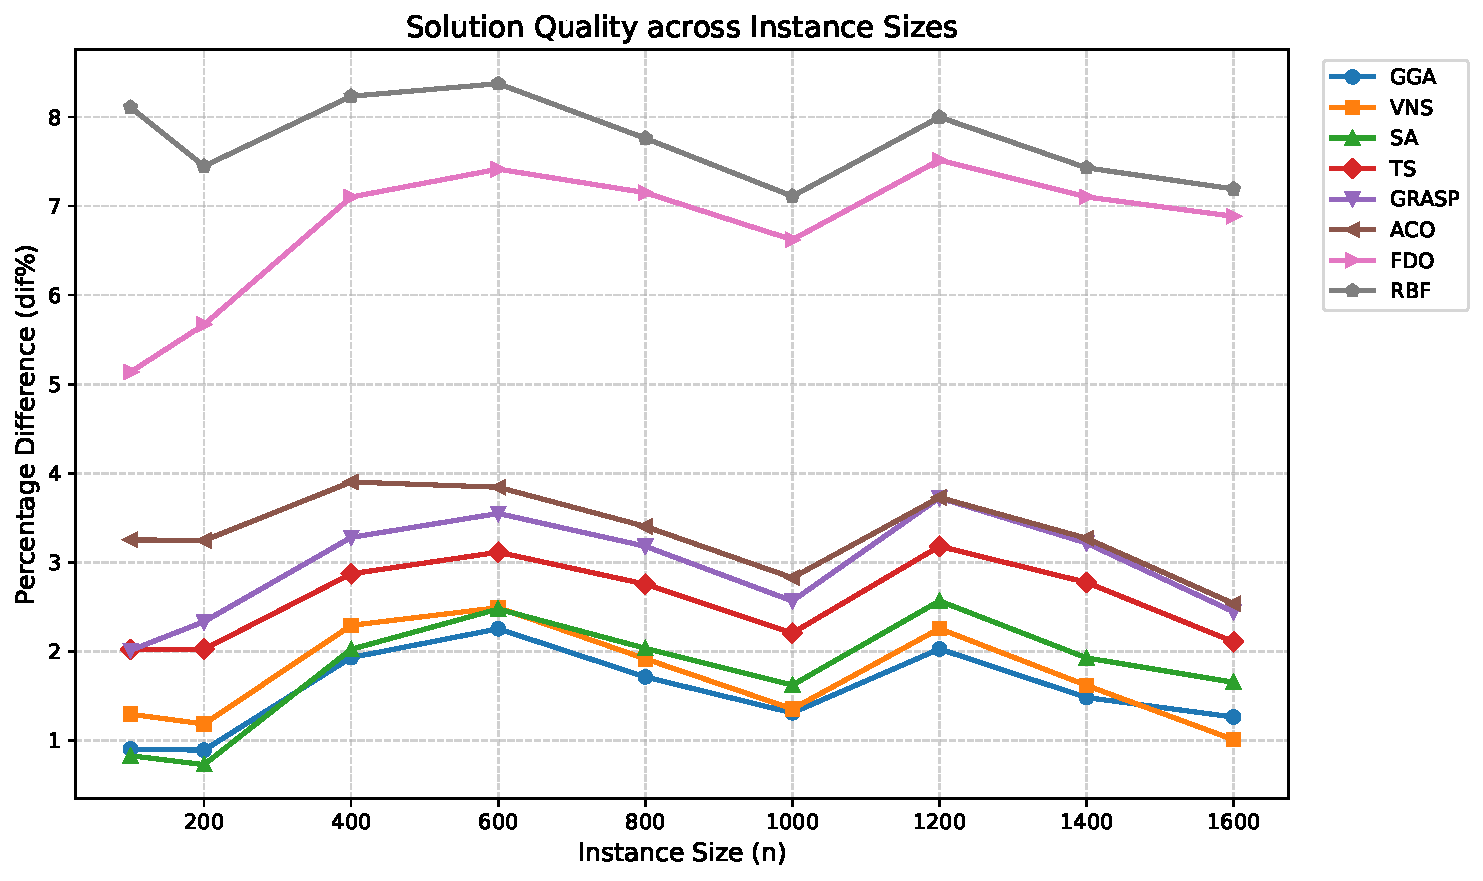
\includegraphics[width=0.85\textwidth]{figures/solution_quality_plot.pdf}
    \caption{Average percentage difference (dif\%) from the theoretical lower bound across varying instance sizes.}
    \label{fig:dif_scaling}
\end{figure}

The execution time profiles reveal an equally important dimension of algorithmic performance. SA's execution time remains remarkably flat, hovering reliably between 15 and 20 seconds regardless of instance size, a direct consequence of its fixed iteration budget discussed above. TS and GRASP scale more gently than the population-based methods, as their fixed iteration budgets directly bound their runtime. The modest growth observed reflects slightly more expensive bin operations as average bin occupancy increases with instance size. GGA's aggressive scaling is driven by its rearrangement by pairs repair heuristic, which must process all free items against all active bins following every crossover and mutation operation. ACO's scaling is similarly steep, as the pheromone matrix grows with the number of distinct item weights in the instance. FDO's scaling mirrors GGA and ACO, driven primarily by the cost of deep-copying solution structures during each iteration, which scales directly with solution size. VNS exhibits a notable spike at $n=1200$ before dropping back at $n=1600$, likely reflecting variance in instance difficulty rather than any systematic algorithmic change. RBF remains near-instantaneous throughout, though this speed advantage is entirely offset by its poor solution quality.

\begin{figure}[H]
    \centering
    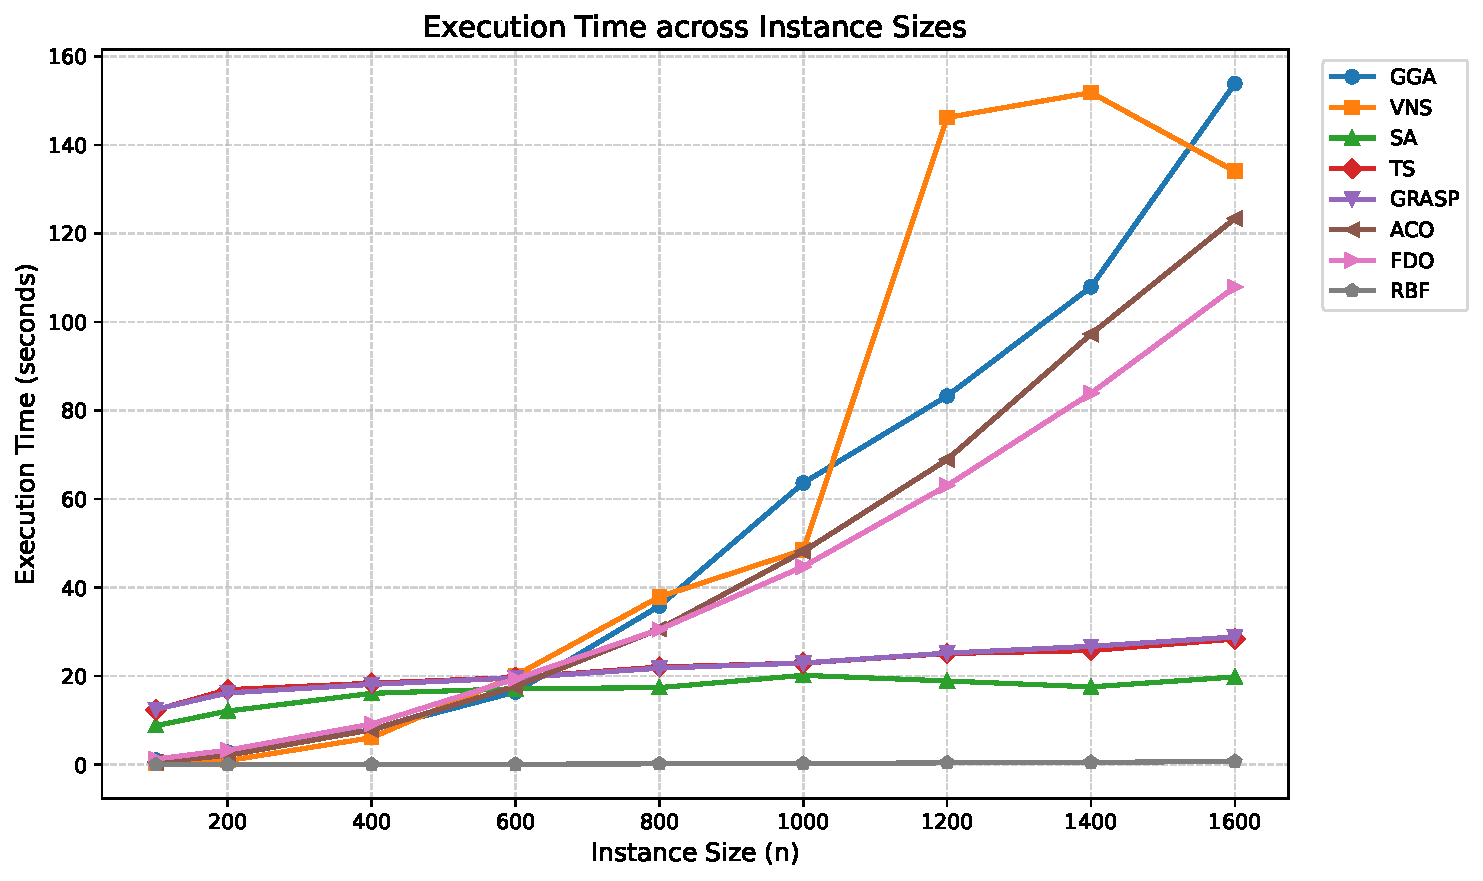
\includegraphics[width=0.85\textwidth]{figures/execution_time_plot.pdf}
    \caption{Average execution time in seconds across varying instance sizes.}
    \label{fig:time_scaling}
\end{figure}

Among the evaluated algorithms, GGA achieves the strongest solution quality overall but incurs substantially higher computational cost at scale, reaching 102 seconds at $n=1600$. SA offers the most favourable balance of quality and efficiency, remaining closely competitive with GGA while maintaining a near-flat execution time profile throughout, making it the more practical choice for large instances. These results establish the relative capability of each human-crafted implementation, providing the baseline against which the LLM-generated variants are directly compared in 
Section~\ref{sec:llm-eval}.

\section{LLM Algorithm Generation Methodology}

\subsection{Model Selection}
To accurately assess the current frontier of automated algorithm design, we selected two state-of-the-art Large Language Models (LLMs): OpenAI's GPT-5.2 and Anthropic's Claude Opus 4.6. At the time of testing (February 2026), these represented the flagship models from their respective organizations and are widely regarded as industry leaders for code generation, consistently ranking at the top of comprehensive leaderboards such as SWE-bench \cite{swebench}. While focusing on proprietary flagship models obscures the exact composition of their training data—unlike open-source alternatives such as StarCoder2 \cite{starcoder2}—it aligns with our primary goal of evaluating the maximum theoretical capability of current AI tools for operations research tasks. 

We initially planned to include Google's Gemini 3 Pro in our evaluation suite. However, because its highest-tier code generation capabilities inherently enforce continuous reasoning tokens that drastically increase API costs, conducting the full iterative testing pipeline across all algorithms became financially prohibitive, and it was subsequently excluded from the final comparison.

\subsection{Prompt Engineering Strategy}
All interactions with the selected LLMs were conducted programmatically via their respective APIs. While recent models exhibit less sensitivity to prompt phrasing \cite{wangz}, systematic prompt engineering remains important. 

We employed a zero-shot prompting strategy, meaning no prior examples of Bin Packing metaheuristics were provided. This simulates the most natural human-computer interaction pattern and avoids biasing the LLM toward specific implementation styles. Furthermore, literature suggests that zero-shot prompting can sometimes outperform few-shot prompting in advanced models, as the LLM focuses purely on the task constraints rather than overfitting to the narrative style of the provided examples \cite{reynolds}.

To maximize reasoning quality, we integrated Chain-of-Thought (CoT) prompting by appending the phrase "Let's think step by step" to the instructions \cite{kojima2022}. We utilize this technique because CoT has been shown to yield clear improvements over direct prompting specifically for code generation tasks \cite{li2024structured}. It is worth noting that while Li et al. \cite{li2024structured} also introduce a more advanced structured approach to CoT, that specific method requires providing input-output examples and explicit test requirements, making it inapplicable to our zero-shot pipeline. Therefore, we rely on the baseline CoT prompt.

Additionally, we utilized persona adoption, instructing the LLM to act as a "senior algorithm designer". While role-playing has been shown to potentially improve reasoning ability \cite{roleplay}, we found no compelling evidence in the literature that it enhances code generation. However, since there is also no evidence suggesting it degrades performance \cite{khojah2025}, we included it as a standard practice. Furthermore, to aid the models in arriving at correct executables, the required Python function signature was provided in the prompt. This has been demonstrated to decrease the probability of encountering ImportErrors and TypeErrors in generated code \cite{khojah2025}. Finally, the generation temperature for both models was left at their default values, as temperature primarily correlates with incoherence rather than algorithmic novelty \cite{peeperkorn}.

\subsection{Iterative Generation and Refinement Pipeline}
To move beyond naive single-prompt generation, we implemented an automated iterative refinement pipeline inspired by the PerfCodeGen framework \cite{perfcodegen}. For every target algorithm, each LLM was allocated $n = 3$ independent candidate runs. To manage API costs, each run has a prompt budget of $p = 5$. 

The pipeline for a single candidate run operates in two distinct phases:
\begin{enumerate}
    \item Correctness Loop: The initial zero-shot prompt requests the complete Python algorithm. The generated code is extracted and executed against a validation suite. If the code throws an execution error or violates constraints (e.g., returning invalid data types), the error traceback is fed back to the LLM in a subsequent prompt with instructions to fix the bug. The algorithm must also abide by a provided time limit (in seconds). If the execution exceeds this allocated time, the generation is classed as incorrect, and a timeout error is fed back to the LLM for correction. This loop repeats until the code executes successfully within all constraints or the prompt budget $p$ is exhausted.
    \item Performance Loop: Once a syntactically correct and executable algorithm is generated, its baseline performance is evaluated on our standard parameter-tuning dataset (test-u), which consists of 10 instances of 400 items and 10 instances of 800 items. The algorithm is constrained by a time limit of $\frac{1}{600}$th of a second per item. Given the composition of the dataset, this equates to a 20-second cumulative time limit across all 20 instances. To provide a slight safety measure against anomalously lucky runs without adding excessive computational overhead, this evaluation is repeated twice. The performance metric we optimise is the Percentage Difference (dif\%) from the theoretical lower bound across the instances. This ensures the selection process specifically favors the code variant that consistently approximates the optimal solution. The subsequent refinement steps depend on the remaining prompt budget. If only one prompt remains, the LLM is provided the code alongside its performance results and asked directly to improve it. If two or more prompts remain, the first refinement iteration is split across two prompts: one asking the LLM to generate a strategic refinement plan based on the performance data, and a second asking it to apply that specific plan. For all subsequent iterations in the loop, this process is condensed: we provide the latest performance feedback and simply ask the LLM to improve the code.
\end{enumerate}
Throughout the performance loop, newly generated code is continually validated for correctness. If an optimization attempt breaks the code, the pipeline discards the broken version and reverts to the most performant correct version for the next prompt. At the conclusion of the $n=3$ candidate runs, the single highest-performing correct algorithm across all runs is selected as the LLM's final submission for that specific metaheuristic.

\section{Evaluation of LLM-Generated Algorithms \label{sec:llm-eval}}

To evaluate the generative capabilities of the selected models, we tested the LLM-generated algorithms against standard benchmark instances from BPPLIB (Falkenauer and Scholl). Because the optima are known for these datasets, the dif\% metric is calculated exactly as before but uses the known optimal rather than the theoretical lower bound. The new opt. metric denotes the total number of instances where an algorithm discovered the optimal solution in at least one of its five independent runs. Randomised Best Fit is excluded from this comparison, as its trivial structure leaves no meaningful implementation design space — any correct implementation produces equivalent results.

\begin{table}[H]
\centering
\caption{Summary of weighted average dif\% from the known optimal across all algorithm variants. Bold indicates best performance per row.}
\label{tab:summary-comparison}
\begin{tabular}{l ccc}
\toprule
Algorithm & Human & Anthropic & OpenAI \\
\midrule
GGA   & 0.16          & \textbf{0.15} & 0.87 \\
SA    & 0.59          & \textbf{0.13} & 0.86 \\
TS    & 0.69          & \textbf{0.25} & 1.51 \\
GRASP & 0.88          & \textbf{0.63} & 0.98 \\
VNS   & 0.60          & 0.58          & \textbf{0.38} \\
ACO   & 1.44          & 1.03          & \textbf{0.81} \\
FDO   & 2.36          & \textbf{0.50} & 0.84 \\
\end{tabular}
\end{table}

Table~\ref{tab:summary-comparison} presents the weighted average dif\% from the known optimal across all evaluated algorithms, providing a macro-level view of performance. Claude Opus 4.6 generated implementations that matched or outperformed the human baseline across all seven algorithms, achieving the lowest deviation in five of them. OpenAI's GPT-5.2 achieved the strongest results on VNS and ACO, outperforming both the human and Anthropic baselines on those two algorithms, but underperformed relative to the human baseline on GGA, SA, TS, and GRASP.

The contrast between algorithms is notable. For GGA, where the human implementation was already highly competitive at 0.16\%, Anthropic matched this closely at 0.15\% while OpenAI struggled significantly at 0.87\%, suggesting difficulty synthesising the group-level encoding and repair mechanisms required by grouping genetic algorithms.

\subsection{Genetic Algorithm (GA)}
% ============================================================
% GGA
% ============================================================
\begin{table}[H]
\centering
\caption{Results obtained by Genetic Algorithm (GA) variants applied to BPP.}
\label{tab:ga-comparison}
\begin{tabular}{l c cc cc cc}
\toprule
\multirow{2}{*}{Class} & \multirow{2}{*}{Inst.} & \multicolumn{2}{c}{GGA} & \multicolumn{2}{c}{Anthropic-GA} & \multicolumn{2}{c}{OpenAI-GA} \\
\cmidrule(lr){3-4} \cmidrule(lr){5-6} \cmidrule(lr){7-8}
 & & opt. & dif \% & opt. & dif \% & opt. & dif \% \\
\midrule
falkenauer-120  & 20   & 20   & 0.12 & 18   & 0.29 & 11   & 1.24 \\
falkenauer-250  & 20   & 15   & 0.30 & 14   & 0.38 & 0    & 1.35 \\
falkenauer-500  & 20   & 10   & 0.42 & 10   & 0.31 & 0    & 1.14 \\
falkenauer-1000 & 20   & 0    & 1.32 & 7    & 0.26 & 0    & 1.04 \\
scholl-10       & 10   & 8    & 0.36 & 8    & 0.47 & 0    & 4.46 \\
scholl-480      & 480  & 438  & 0.23 & 434  & 0.22 & 299  & 1.58 \\
scholl-720      & 720  & 672  & 0.08 & 674  & 0.08 & 592  & 0.32 \\
\midrule
Total           & 1290 & 1163 &      & 1165 &      & 902  &      \\
Weighted Avg    &      &      & 0.16 &      & 0.15 &      & 0.87 \\
\bottomrule
\end{tabular}
\end{table}

Anthropic's implementation marginally outperformed the human baseline, discovering 1165 optimal solutions compared to 1163 and reducing the weighted average dif\% from 0.16\% to 0.15\%. OpenAI's implementation struggled significantly, finding only 902 optimal solutions with a weighted average dif\% of 0.87\%.

The three implementations differ substantially in their choice of representation. The 
human uses a true grouping genetic algorithm with bin-level encoding throughout: 
crossover operates directly on bin groups, and a repair heuristic handles any items 
left unassigned after recombination. Anthropic uses permutation encoding decoded via 
BFD, with a BPX crossover that partially preserves bin structure by alternately 
inheriting the fullest bins from each parent, followed by a post-decode local search 
that attempts to empty the lightest bins. OpenAI uses continuous random-key encoding 
decoded to an item ordering, the most indirect representation of the three, with blend 
and OX crossover operating on the key vectors rather than on bin structure directly.

The human's group-level encoding appears to provide an advantage on the falkenauer 
classes, where it outperforms Anthropic on the smaller instances. Anthropic recovers 
on the larger falkenauer-1000 class, where its post-decode local search and diverse 
initialisation appear to compensate. OpenAI's poor performance is consistent with the 
known difficulty of indirect encodings on grouping problems --- without operators that 
explicitly preserve or exploit bin structure, the search struggles to discover and 
maintain high-quality groupings.

\subsection{Simulated Annealing (SA)}
% ============================================================
% SA
% ============================================================
\begin{table}[H]
\centering
\caption{Results obtained by Simulated Annealing (SA) variants applied to BPP.}
\label{tab:sa-comparison}
\begin{tabular}{l c cc cc cc}
\toprule
\multirow{2}{*}{Class} & \multirow{2}{*}{Inst.} & \multicolumn{2}{c}{SA} & \multicolumn{2}{c}{Anthropic-SA} & \multicolumn{2}{c}{OpenAI-SA} \\
\cmidrule(lr){3-4} \cmidrule(lr){5-6} \cmidrule(lr){7-8}
 & & opt. & dif \% & opt. & dif \% & opt. & dif \% \\
\midrule
falkenauer-120  & 20   & 6    & 1.44 & 20   & 0.16 & 6    & 1.44 \\
falkenauer-250  & 20   & 0    & 1.48 & 12   & 0.46 & 0    & 1.47 \\
falkenauer-500  & 20   & 0    & 1.34 & 3    & 0.56 & 0    & 1.32 \\
falkenauer-1000 & 20   & 0    & 0.94 & 0    & 0.73 & 0    & 1.18 \\
scholl-10       & 10   & 8    & 0.36 & 8    & 0.36 & 0    & 3.70 \\
scholl-480      & 480  & 397  & 0.69 & 455  & 0.12 & 310  & 1.32 \\
scholl-720      & 720  & 546  & 0.44 & 650  & 0.10 & 561  & 0.45 \\
\midrule
Total           & 1290 & 957  &      & 1148 &      & 877  &      \\
Weighted Avg    &      &      & 0.59 &      & 0.13 &      & 0.86 \\
\bottomrule
\end{tabular}
\end{table}

Anthropic's Claude Opus 4.6 outperformed the human baseline, discovering 1148 
optimal solutions compared to the human's 957 and reducing the weighted average dif\% 
from 0.59\% to 0.13\%. The key implementation difference is the cooling schedule. 
Rather than using a fixed $\alpha$, the generated SA estimates the number of available 
iterations from the remaining time budget and computes $\alpha$ dynamically, then 
recalibrates the temperature against wall-clock progress every 500 iterations. This 
makes it more responsive, allowing it to better utilise the available time budget across different instance sizes.

GPT-5.2 underperformed the human baseline, yielding only 877 optimal solutions and a 
higher deviation of 0.86\%. The root cause is a fundamental flaw in the objective 
function. OpenAI's implementation scores feasible solutions as 
$\text{bins\_used} \times M + \text{total\_slack} \times 0.01$, where 
$M = C \times (n + 5)$. The $\text{bins\_used} \times M$ term only changes when a bin 
is eliminated entirely. The $\text{total\_slack} \times 0.01$ term is conserved across 
all feasible moves, moving an item from one bin to another gains exactly as much 
slack in the source bin as it loses in the destination. Consequently, the objective 
function returns an identical value for the majority of moves, so fails to guide the search. The algorithm cannot distinguish between a tightly packed solution on the verge of bin elimination and one where items are spread evenly across bins, reducing it to a near-random walk with only occasional improvement when a bin is eliminated by chance.

\subsection{Variable Neighbourhood Search}
% ============================================================
% VNS
% ============================================================
\begin{table}[H]
\centering
\caption{Results obtained by Variable Neighbourhood Search (VNS) variants applied to BPP.}
\label{tab:vns-comparison}
\begin{tabular}{l c cc cc cc}
\toprule
\multirow{2}{*}{Class} & \multirow{2}{*}{Inst.} & \multicolumn{2}{c}{VNS} & \multicolumn{2}{c}{Anthropic-VNS} & \multicolumn{2}{c}{OpenAI-VNS} \\
\cmidrule(lr){3-4} \cmidrule(lr){5-6} \cmidrule(lr){7-8}
 & & opt. & dif \% & opt. & dif \% & opt. & dif \% \\
\midrule
falkenauer-120  & 20   & 15   & 0.70 & 10   & 1.03 & 17   & 0.63 \\
falkenauer-250  & 20   & 7    & 0.88 & 0    & 1.23 & 9    & 0.78 \\
falkenauer-500  & 20   & 1    & 0.82 & 0    & 1.03 & 0    & 0.75 \\
falkenauer-1000 & 20   & 0    & 0.78 & 0    & 0.81 & 0    & 0.85 \\
scholl-10       & 10   & 0    & 2.96 & 0    & 2.60 & 8    & 0.57 \\
scholl-480      & 480  & 356  & 1.14 & 335  & 0.91 & 406  & 0.61 \\
scholl-720      & 720  & 629  & 0.19 & 592  & 0.28 & 632  & 0.18 \\
\midrule
Total           & 1290 & 1008 &      & 937  &      & 1072 &      \\
Weighted Avg    &      &      & 0.60 &      & 0.58 &      & 0.38 \\
\bottomrule
\end{tabular}
\end{table}

OpenAI's GPT-5.2 outperformed both the human baseline and Anthropic's implementation, finding 1072 optimal solutions compared to 1008 and 937 respectively, and achieving a weighted average dif\% of 0.38\% versus 0.60\% and 0.58\%. The gap is most pronounced on the scholl-10 class, where OpenAI discovered 8 optimal solutions while the other implementations found none.

The primary difference lies in the local search strategy. The human implementation uses an exhaustive best-improvement procedure that evaluates all possible item transfers and swaps. In contrast, the OpenAI implementation employs a Variable Neighbourhood Descent with relocate, swap, and a specialised 2-0 neighbourhood that attempts to empty bins by relocating pairs of items simultaneously. This compound move is absent from the other implementations and provides a direct mechanism for bin elimination, which likely contributes to the stronger performance observed across several instance classes.

Anthropic’s implementation achieved a similar weighted average dif\% to the human baseline (0.58\% vs 0.60\%) but found fewer optimal solutions. This is likely because its design places greater emphasis on diversification through multiple shaking operators, whereas the human implementation relies on deeper local exploitation.

\subsection{Tabu Search (TS)}
% ============================================================
% TS
% ============================================================
\begin{table}[H]
\centering
\caption{Results obtained by Tabu Search (TS) variants applied to BPP.}
\label{tab:tabu-comparison}
\begin{tabular}{l c cc cc cc}
\toprule
\multirow{2}{*}{Class} & \multirow{2}{*}{Inst.} & \multicolumn{2}{c}{TS Search} & \multicolumn{2}{c}{Anthropic-TS} & \multicolumn{2}{c}{OpenAI-TS} \\
\cmidrule(lr){3-4} \cmidrule(lr){5-6} \cmidrule(lr){7-8}
 & & opt. & dif \% & opt. & dif \% & opt. & dif \% \\
\midrule
falkenauer-120  & 20   & 6    & 1.44 & 15   & 0.52 & 6    & 1.44 \\
falkenauer-250  & 20   & 0    & 1.48 & 8    & 0.69 & 0    & 1.48 \\
falkenauer-500  & 20   & 0    & 1.33 & 2    & 0.68 & 0    & 1.34 \\
falkenauer-1000 & 20   & 0    & 1.17 & 0    & 0.64 & 0    & 1.21 \\
scholl-10       & 10   & 5    & 1.18 & 5    & 3.60 & 0    & 6.06 \\
scholl-480      & 480  & 353  & 0.96 & 425  & 0.31 & 236  & 3.01 \\
scholl-720      & 720  & 567  & 0.42 & 646  & 0.13 & 547  & 0.47 \\
\midrule
Total           & 1290 & 931  &      & 1101 &      & 789  &      \\
Weighted Avg    &      &      & 0.69 &      & 0.25 &      & 1.51 \\
\bottomrule
\end{tabular}
\end{table}

Anthropic's Claude Opus 4.6 substantially outperformed both the human baseline and the 
OpenAI implementation, discovering 1101 optimal solutions compared to 931 and 789 
respectively, and reducing the weighted average dif\% from 0.69\% to 0.25\%. In 
contrast, OpenAI's GPT-5.2 underperformed the human baseline on nearly all instance 
classes and performed particularly poorly on the scholl-10 and 
scholl-480 sets.

The most notable structural difference between the implementations is Anthropic's 
adoption of an iterative bin-reduction strategy. While the human and OpenAI 
implementations perform conventional feasibility-preserving tabu search starting from 
a valid packing, the Anthropic implementation repeatedly attempts to reduce the number 
of bins by constructing an intentionally infeasible packing and then applying tabu 
search to minimise overflow until feasibility is restored. This gives the search a 
clear objective at each stage, eliminating overflow, rather than relying on 
gradual improvements that only materialise when a bin happens to empty entirely. 

The human and OpenAI implementations differ from each other primarily in their 
bin-targeting strategy: the human concentrates around 60\% of relocate moves on the 
single emptiest bin, creating sustained pressure toward eliminating it, whereas OpenAI 
distributes attention across the lightest third of bins, which is less likely to fully 
empty any individual bin.

\subsection{Greedy Randomised Adaptive Search Procedure (GRASP)}
% ============================================================
% GRASP
% ============================================================
\begin{table}[H]
\centering
\caption{Results obtained by GRASP variants applied to BPP.}
\label{tab:grasp-comparison}
\begin{tabular}{l c cc cc cc}
\toprule
\multirow{2}{*}{Class} & \multirow{2}{*}{Inst.} & \multicolumn{2}{c}{GRASP} & \multicolumn{2}{c}{Anthropic-GRASP} & \multicolumn{2}{c}{OpenAI-GRASP} \\
\cmidrule(lr){3-4} \cmidrule(lr){5-6} \cmidrule(lr){7-8}
 & & opt. & dif \% & opt. & dif \% & opt. & dif \% \\
\midrule
falkenauer-120  & 20   & 5    & 1.72 & 16   & 0.51 & 14   & 0.74 \\
falkenauer-250  & 20   & 0    & 1.53 & 6    & 0.90 & 5    & 0.99 \\
falkenauer-500  & 20   & 0    & 1.41 & 0    & 1.10 & 0    & 1.06 \\
falkenauer-1000 & 20   & 0    & 1.33 & 0    & 1.09 & 0    & 1.04 \\
scholl-10       & 10   & 1    & 2.10 & 0    & 4.74 & 0    & 4.82 \\
scholl-480      & 480  & 317  & 1.33 & 366  & 1.17 & 299  & 2.04 \\
scholl-720      & 720  & 540  & 0.50 & 629  & 0.17 & 620  & 0.22 \\
\midrule
Total           & 1290 & 863  &      & 1017 &      & 938  &      \\
Weighted Avg    &      &      & 0.88 &      & 0.63 &      & 0.98 \\
\bottomrule
\end{tabular}
\end{table}

Anthropic's implementation outperformed both the human baseline and OpenAI, discovering 1017 optimal solutions compared to 863 and 938 respectively, and reducing the weighted average dif\% from 0.88\% to 0.63\%. The key structural difference from the human baseline is in the local search: Anthropic uses a greedy bin-emptying procedure that repeatedly attempts to relocate all items from the lightest bin via best-fit, falling back to 1-1 swaps when direct emptying fails, whereas the human uses a tabu-based local search. Anthropic performs worse than the human only on scholl-10, where tabu-based search appears better suited to the small instance size.

OpenAI discovered more optimal solutions than the human baseline (938 vs 863) but 
registered a higher weighted average dif\% (0.98\% vs 0.88\%), and underperformed 
Anthropic on both metrics. Its local search is the richest of the three, incorporating 
beam emptying, ejection chains, and large neighbourhood repack, yet this does not 
translate to stronger average-case performance. The most notable result is scholl-480, 
where OpenAI performs substantially worse than both other implementations.

\subsection{Ant Colony Optimisation (ACO)}
% ============================================================
% ACO
% ============================================================
\begin{table}[H]
\centering
\caption{Results obtained by Ant Colony Optimisation (ACO) variants applied to BPP.}
\label{tab:aco-comparison}
\begin{tabular}{l c cc cc cc}
\toprule
\multirow{2}{*}{Class} & \multirow{2}{*}{Inst.} & \multicolumn{2}{c}{ACO} & \multicolumn{2}{c}{Anthropic-ACO} & \multicolumn{2}{c}{OpenAI-ACO} \\
\cmidrule(lr){3-4} \cmidrule(lr){5-6} \cmidrule(lr){7-8}
 & & opt. & dif \% & opt. & dif \% & opt. & dif \% \\
\midrule
falkenauer-120  & 20   & 4    & 1.96 & 15   & 0.86 & 14   & 0.88 \\
falkenauer-250  & 20   & 0    & 2.01 & 2    & 1.06 & 3    & 1.04 \\
falkenauer-500  & 20   & 0    & 1.77 & 0    & 1.04 & 0    & 0.89 \\
falkenauer-1000 & 20   & 0    & 1.64 & 0    & 1.07 & 0    & 0.89 \\
scholl-10       & 10   & 0    & 5.95 & 0    & 5.06 & 0    & 4.92 \\
scholl-480      & 480  & 256  & 2.37 & 289  & 2.18 & 319  & 1.59 \\
scholl-720      & 720  & 503  & 0.71 & 619  & 0.21 & 623  & 0.21 \\
\midrule
Total           & 1290 & 763  &      & 925  &      & 959  &      \\
Weighted Avg    &      &      & 1.44 &      & 1.03 &      & 0.81 \\
\bottomrule
\end{tabular}
\end{table}

Both LLM implementations outperformed the human baseline, which discovered 763 optimal solutions with a weighted average dif\% of 1.44\%. OpenAI achieved the 
strongest overall result, finding 959 optimal solutions and a weighted average dif\% of 0.81\%, with Anthropic close behind at 925 and 1.03\%.

ACO is sufficiently computationally expensive that all implementations complete very 
few iterations within the time budget. This allows for very few pheromone update cycles, so trail differentiation from initial values is minimal, and performance is driven primarily by single-construction quality rather than accumulated pheromone learning. This means the results reflect early-stage behaviour rather than the algorithm operating as intended.

On smaller instances the human's hard cap of 20 ant constructions leaves the time 
budget largely unused, which likely explains the large gap on falkenauer-120. On larger instances the time budget is exhausted, yet the human still underperforms. Since pheromone learning is limited across all implementations, construction quality is the most plausible explanation. OpenAI's construction includes a look-ahead that rewards placing an item in a bin if the remaining capacity afterwards is exactly fillable by another unpacked item, directly targeting tight bin filling at each step. OpenAI also evaluates more ants per iteration than Anthropic across all instance sizes, producing greater construction diversity within the available time. These factors are the most plausible explanation for OpenAI's stronger performance.

\subsection{Fitness dependent optimiser (FDO)}
% ============================================================
% FDO
% ============================================================
\begin{table}[H]
\centering
\caption{Results obtained by Fitness Dependent Optimizer (FDO) variants applied to BPP.}
\label{tab:fdo-comparison}
\begin{tabular}{l c cc cc cc}
\toprule
\multirow{2}{*}{Class} & \multirow{2}{*}{Inst.} & \multicolumn{2}{c}{FDO} & \multicolumn{2}{c}{Anthropic-FDO} & \multicolumn{2}{c}{OpenAI-FDO} \\
\cmidrule(lr){3-4} \cmidrule(lr){5-6} \cmidrule(lr){7-8}
 & & opt. & dif \% & opt. & dif \% & opt. & dif \% \\
\midrule
falkenauer-120  & 20   & 0    & 3.61 & 15   & 0.72 & 8    & 1.36 \\
falkenauer-250  & 20   & 0    & 4.15 & 6    & 0.86 & 0    & 1.32 \\
falkenauer-500  & 20   & 0    & 4.39 & 0    & 0.89 & 0    & 1.28 \\
falkenauer-1000 & 20   & 0    & 4.59 & 0    & 0.64 & 0    & 1.21 \\
scholl-10       & 10   & 0    & 6.91 & 0    & 2.71 & 0    & 5.49 \\
scholl-480      & 480  & 238  & 2.47 & 361  & 0.88 & 309  & 1.45 \\
scholl-720      & 720  & 306  & 2.01 & 639  & 0.18 & 590  & 0.32 \\
\midrule
Total           & 1290 & 544  &      & 1021 &      & 907  &      \\
Weighted Avg    &      &      & 2.36 &      & 0.50 &      & 0.84 \\
\bottomrule
\end{tabular}
\end{table}

The human baseline struggled considerably with FDO, discovering only 544 optimal 
solutions and recording the highest weighted average dif\% of any algorithm in this 
study at 2.36\%. The core difficulty lies in translating FDO's continuous velocity 
concept to a discrete domain: the human implementation maps velocity directly to item 
transfers between bins, discarding any infeasible moves. 

OpenAI's implementation instead preserves the continuous velocity update $\Delta x = r \cdot fw \cdot (\text{leader} - x)$ applied to priority vectors that are decoded into packings via BFD. This retains the core FDO mechanic while mapping it to a discrete representation in a well-defined way. It discovered 907 optimal solutions and a weighted average dif\% of 0.84\%, comfortably outperforming the human baseline on both metrics.

Anthropic's implementation achieves the strongest numerical result --- 1021 optimal 
solutions and 0.50\% --- but its classification as an FDO implementation is 
questionable. While it computes a fitness weight $fw$ and uses it to select between 
operator pools, the movement operators themselves are OX crossover, segment reversals, 
block insertions, and position swaps toward the best solution. This is more 
characteristic of a permutation-based evolutionary algorithm than FDO, and its 
superior performance may reflect the suitability of that paradigm for the BPP rather 
than the quality of the FDO translation. For this reason, OpenAI's implementation is 
the more meaningful point of comparison against the human baseline in this category.

\section{Discussion}

\subsection{Human-Implemented Algorithms}

The results from Section 4 provide a clear answer to the first research question. GGA 
and SA consistently outperformed the other implementations, with GGA achieving the 
strongest solution quality overall and SA offering the most favourable balance of 
quality and computational efficiency. The mid-tier cluster of TS, GRASP, VNS, and ACO 
produced broadly comparable results, while FDO and RBF were consistently the weakest 
performers. The poor relative performance of ACO and FDO is largely attributable to 
computational constraints rather than inherent algorithmic weakness --- both are 
population-based methods whose core mechanics require sufficient iterations to operate 
as intended, and neither received enough time to do so within the allocated budget. 
This is an important caveat when interpreting their rankings.

\subsection{LLM-Generated Algorithms}

The results in Section 6 provide a broadly positive answer to the second research question. Both LLMs produced functionally correct implementations for all seven algorithms, and both frequently matched or exceeded human-level performance. Anthropic's Claude Opus 4.6 matched or outperformed the human baseline across all seven algorithms, achieving the best result in five of them. This is a strong result, particularly given the zero-shot generation strategy employed. The Anthropic SA implementation is especially notable: rather than using a fixed cooling parameter, it adopts a dynamic schedule that adapts to the available time budget, producing a more effective implementation than the human's fixed-parameter approach. Similarly, the Anthropic TS 
implementation uses an iterative bin-reduction formulation rather than conventional feasibility-preserving search, which proved substantially more effective on the benchmark instances. In both cases the human implementation did not employ these approaches, and the performance gap reflects this difference in design.

However, the results also reveal clear limitations. OpenAI's SA implementation contained a fundamental flaw in its objective function that rendered the search almost entirely uninformative, and its TS implementation underperformed the human baseline across nearly 
all instance classes. These failures were not syntactic --- the code executed correctly and produced valid packings --- but reflect deeper reasoning errors in algorithm design. This distinction is important: correctness and performance are separable, and the iterative pipeline's correctness loop cannot detect the latter.

\subsection{Patterns Across LLMs}

Addressing the third research question, the two models exhibit distinct strengths and 
weaknesses. Anthropic performs more consistently across the full suite, producing 
competitive implementations for every algorithm. OpenAI shows higher variance: it 
achieves the strongest results on VNS and ACO, where construction-level decisions and 
neighbourhood structure appear to play to its strengths, but struggles considerably on 
TS and SA where a precise understanding of the objective function is critical. The SA 
objective function flaw in particular suggests that OpenAI may be more prone to 
plausible-looking but subtly incorrect implementations that pass correctness checks 
while failing to guide the search effectively.

A recurring theme across both models is the tendency to deviate from the specified 
algorithm paradigm when a more familiar or effective approach is available. This was 
most pronounced in Anthropic's FDO implementation, which adopted permutation-based 
evolutionary operators rather than a genuine FDO velocity translation, and to a lesser 
degree in both LLM GA implementations, which used permutation encoding rather than the 
group-level encoding central to the GGA paradigm. Whether this constitutes a failure 
depends on how the task is framed: if the goal is to produce the best-performing 
algorithm, paradigm deviation may be acceptable or even desirable; if the goal is to 
evaluate a specific algorithm's generative capability, it undermines the comparison.

\subsection{Limitations}

Several limitations of this study warrant acknowledgement. First, only two LLMs were 
evaluated. The planned inclusion of Google's Gemini 3 Pro was excluded on cost grounds, 
which restricts the generalisability of conclusions about inter-model differences. 
Second, the zero-shot prompting strategy, while methodologically clean, does not 
represent the upper bound of LLM capability --- few-shot prompting or human-in-the-loop 
refinement may yield substantially stronger results. Third, the iterative pipeline 
selects the best-performing candidate across three independent runs evaluated on a 
fixed tuning dataset; this introduces a degree of optimistic selection bias, 
particularly for high-variance implementations. Fourth, all implementations were 
written in Python, which imposes computational constraints that disproportionately 
affect iteration-heavy algorithms such as ACO and FDO. A compiled language 
implementation might substantially alter the relative rankings of these algorithms. 
Finally, the LLM evaluation used only the Falkenauer and Scholl benchmark classes from 
BPPLIB. While these are standard and well-regarded, they represent a specific 
distribution of instance structure, and performance on other benchmark families may 
differ.

\subsection{Future Work}

Several directions present themselves as natural extensions of this study. The BPP is 
a well-studied problem with a substantial body of published implementations, meaning 
the models may have had direct or indirect exposure to relevant design patterns during 
training. Evaluating LLM-generated metaheuristics on harder or less well-documented 
combinatorial problems --- such as the 2D bin packing problem or vehicle routing --- 
would provide a stronger test of genuine algorithmic reasoning ability and reduce the 
confound between knowledge retrieval and algorithmic synthesis. Additionally, both 
models were queried in standard mode; reasoning-augmented variants, which allow 
extended internal deliberation before generating a response, were excluded due to cost 
constraints but may produce meaningfully different results, particularly for algorithms 
where subtle design choices have an outsized impact on performance. Finally, 
reimplementing the full suite in a compiled language would remove the computational 
bottleneck that disproportionately affects ACO and FDO, potentially revealing a more 
accurate picture of their relative algorithmic strength.

\section{Conclusion}

This study evaluated a diverse suite of human-implemented randomised algorithms for 
the 1D Bin Packing Problem and compared them against zero-shot implementations generated by two state-of-the-art LLMs. Across all three research questions, the results yield clear and practically meaningful findings.

Among the human-implemented algorithms, GGA achieved the strongest solution quality overall, with SA offering the most practical balance of quality and computational efficiency. The remaining algorithms formed a broadly comparable mid-tier, with ACO and FDO constrained by the computational overhead of their population based mechanics rather than any fundamental algorithmic weakness.

The LLM evaluation produced results that are both impressive and instructive. Anthropic's Claude Opus 4.6 matched or outperformed the human baseline across all seven algorithms, with several implementations incorporating design choices that the human baseline did not. The dynamic cooling schedule in its SA implementation and the iterative bin-reduction framework in its TS implementation are both well-established techniques in the literature that the human implementation did not employ, and their inclusion contributed meaningfully to the performance advantage. OpenAI's GPT-5.2 showed stronger variance, achieving the best results on VNS and ACO while failing to match the human baseline on TS and SA. The SA objective function flaw illustrates a category of failure that is particularly difficult to detect automatically: the code is correct, the search runs, and valid packings are produced, but the algorithm is not actually doing what it claims to.

The FDO results raise a broader question about what it means to evaluate LLM-generated algorithm implementations. Anthropic's implementation achieved the strongest numerical result in that category but is more accurately described as a permutation-based evolutionary algorithm than an FDO translation. This ambiguity --- where an LLM produces a better-performing algorithm than the one requested --- is likely to recur as these models become more capable, and future evaluation frameworks will need to decide explicitly whether paradigm fidelity or empirical performance is the primary criterion.

Overall, the findings suggest that flagship LLMs are now capable of producing competitive metaheuristic implementations from scratch, drawing on a broad knowledge of existing techniques to assemble implementations that compare favourably with carefully tuned human baselines. However, they remain capable of subtle but consequential reasoning errors that pass all correctness checks while undermining the search. For practitioners, this implies that LLM-generated optimisation code should be treated as a strong starting point requiring algorithmic review, rather than a finished product.

\begin{thebibliography}{00}
\bibitem{maxence} Maxence Delorme, Manuel Iori, Silvano Martello, Bin packing and cutting stock problems: Mathematical models and exact algorithms, European Journal of Operational Research, Volume 255, Issue 1, 2016, Pages 1-20, ISSN 0377-2217, \url{https://doi.org/10.1016/j.ejor.2016.04.030}.

\bibitem{munien} Munien, Chanaleä and Ezugwu, Absalom E.. "Metaheuristic algorithms for one-dimensional bin-packing problems: A survey of recent advances and applications" Journal of Intelligent Systems, vol. 30, no. 1, 2021, pp. 636-663. \url{https://doi.org/10.1515/jisys-2020-0117}

\bibitem{garey} Garey, Michael R. and Johnson, David S. Computers and Intractability: A Guide to the Theory of NP-Completeness. W. H. Freeman, 1979.

\bibitem{sean} Sean Luke, 2013, Essentials of Metaheuristics, Lulu, second edition, available for free at \url{https://people.cs.gmu.edu/~sean/book/metaheuristics/Essentials.pdf}

\bibitem{yang} Yang, X.-S. (2011). Metaheuristic Optimization. Scholarpedia, 6 (8), 11472. \url{https://doi.org/10.4249/scholarpedia.11472}

\bibitem{kucharavy} Kucharavy, A. (2024). Fundamental limitations of generative LLMs. In \textit{Large Language Models in Cybersecurity: Threats, Exposure and Mitigation} (pp. 55--64). Springer Nature Switzerland, Cham. \url{https://library.oapen.org/bitstream/handle/20.500.12657/90897/978-3-031-54827-7.pdf}

\bibitem{chang} Chang Y, Wang X, Wang J, Wu Y, Yang L, Zhu K, Chen H, Yi X, Wang C, Wang Y, Ye W, Zhang Y, Chang Y, Yu PS, Yang Q, Xie X. A Survey on Evaluation of Large Language Models. ACM Trans. Intell. Syst. Technol. 2024;15(3):Article 39 (45 pages). \url{https://doi.org/10.1145/3641289} 

\bibitem{bubeck} Bubeck S, Chandrasekaran V, Eldan R, Gehrke J, Horvitz E, Kamar E, Lee P, Lee YT, Li Y, Lundberg S, Nori H, Palangi H, Ribeiro MT, Zhang Y. Sparks of Artificial General Intelligence: Early experiments with GPT-4. arXiv preprint arXiv:2303.12712. 2023. \url{https://arxiv.org/abs/2303.12712} 

\bibitem{wang} Wang, L., Shi, C., Du, S., Tao, Y., Shen, Y., Zheng, H., \& Qiu, X. (2024). Performance Review on LLM for solving leetcode problems. In 2024 4th International Symposium on Artificial Intelligence and Intelligent Manufacturing (AIIM) (pp. 1050--1054). \url{https://doi.org/10.1109/AIIM64537.2024.10934280} 

\bibitem{coignion} Coignion, T., Quinton, C., \& Rouvoy, R. (2024). A Performance Study of LLM-Generated Code on Leetcode. In Proceedings of the 28th International Conference on Evaluation and Assessment in Software Engineering (pp. 79--89). Association for Computing Machinery, New York, NY, USA. \url{https://doi.org/10.1145/3661167.3661221} 

\bibitem{martello} Silvano Martello, Paolo Toth, Lower bounds and reduction procedures for the bin packing problem, Discrete Applied Mathematics, Volume 28, Issue 1, 1990, Pages 59--70, ISSN 0166-218X, \url{https://doi.org/10.1016/0166-218X(90)90094-S}.

\bibitem{fekete} Fekete, S. \& Schepers, J. New classes of fast lower bounds for bin packing problems. Math. Program. 91, 11--31 (2001). \url{https://doi.org/10.1007/s101070100243} 

\bibitem{BPPLIB} M. Delorme, M. Iori, and S. Martello. BPPLIB: A library for bin packing and cutting stock problems. Optimization Letters, 12(2):235-250, 2018. \url{https://github.com/mdelorme2/BPPLIB}.

\bibitem{gendreau} Gendreau, Michel and Potvin, Jean-Yves, editors. Handbook of Metaheuristics, Third Edition. International Series in Operations Research \& Management Science. Springer, 2019.\url{https://doi.org/10.1007/978-3-319-91086-4}

\bibitem{rajeev} Motwani, R. and Raghavan, P. Randomized Algorithms. 
Cambridge University Press, 1995.

\bibitem{sonuc} Sonuç, E., Şen, B. and Bayır, Ş., 2017. Solving Bin Packing Problem Using Simulated Annealing. In: Proceedings of the 65th ISERD International Conference, Mecca, Saudi Arabia, 23–24 January 2017. World Research Library, pp. 83–85. \url{https://worldresearchlibrary.org/up\_proc/pdf/635-148739346283-85.pdf}

\bibitem{kryz} Krzysztof Fleszar, Khalil S. Hindi, New heuristics for one-dimensional bin-packing, Computers \& Operations Research, Volume 29, Issue 7, 2002, Pages 821-839, ISSN 0305-0548, \url{https://doi.org/10.1016/S0305-0548(00)00082-4}.

\bibitem{lodi} Lodi, A., Martello, S. \& Vigo, D. TSpack: A Unified Tabu Search Code for Multi-Dimensional Bin Packing Problems. Ann Oper Res 131, 203–213 (2004). \url{https://doi.org/10.1023/B:ANOR.0000039519.03572.08}

\bibitem{dosa} D\'osa, G. (2007). The tight bound of First Fit Decreasing bin-packing algorithm is FFD(I) $\leq$ 11/9 OPT(I) + 6/9. In B. Chen, M. Paterson, \& G. Zhang (Eds.), \textit{Combinatorics, Algorithms, Probabilistic and Experimental Methodologies (ESCAPE 2007)} (Lecture Notes in Computer Science, vol.~4614, pp.~1--11). Springer, Berlin, Heidelberg. \url{https://doi.org/10.1007/978-3-540-74450-4\_1}

\bibitem{gga} Falkenauer, E. (1996). The Grouping Genetic Algorithm. In: Floudas, C.A., Pardalos, P.M. (eds) State of the Art in Global Optimization. Nonconvex Optimization and Its Applications, vol 7. Springer, Boston, MA. \url{https://doi.org/10.1007/978-1-4613-3437-8_17}

\bibitem{quirozca} M. Quiroz-Castellanos, L. Cruz-Reyes, J. Torres-Jimenez, C. Gómez S., H. J. Fraire Huacuja, and A. C. F. Alvim. A grouping genetic algorithm with controlled gene transmission for the bin packing problem. Computers \& Operations Research, 55:52-64, 2015. \url{https://doi.org/10.1016/j.cor.2014.10.010}

\bibitem{stuetzle} Stützle, T., \& Hoos, H. H. (2000). MAX–MIN Ant System. Future Generation Computer Systems, 16 (8), 889--914. \url{https://doi.org/10.1016/S0167-739X(00)00043-1}

\bibitem{levine} Levine, J., \& Ducatelle, F. (2004). Ant colony optimization and local search for bin packing and cutting stock problems. Journal of the Operational Research Society, 55(7), 705–716. \url{https://doi.org/10.1057/palgrave.jors.2601771} 

\bibitem{aaron} Aaron C. Zecchin, Angus R. Simpson, Holger R. Maier, Michael Leonard, Andrew J. Roberts, Matthew J. Berrisford, Application of two ant colony optimisation algorithms to water distribution system optimisation, Mathematical and Computer Modelling, Volume 44, Issues 5–6, 2006, Pages 451-468, ISSN 0895-7177, \url{https://doi.org/10.1016/j.mcm.2006.01.005} 

\bibitem{mladenovic} N. Mladenovi{\'c}, P. Hansen, Variable neighborhood search, Computers \& Operations Research, Volume 24, Issue 11, 1997, Pages 1097--1100, ISSN 0305-0548, \url{https://doi.org/10.1016/S0305-0548(97)00031-2}.

\bibitem{gupta} Gupta JND, Ho JC. A new heuristic algorithm for the one-dimensional bin-packing problem. Production Planning \& Control. 1999;10(6):598--603. \url{https://doi.org/10.1080/095372899232894}

\bibitem{abdullah} Abdullah JM, Ahmed T. Fitness Dependent Optimizer: Inspired by the Bee Swarming Reproductive Process. IEEE Access. 2019;7:43473--43486. \url{https://doi.org/10.1109/ACCESS.2019.2907012} 

\bibitem{abdulminaam} Abdul-Minaam DS, Al-Mutairi WMES, Awad MA, El-Ashmawi WH. An Adaptive Fitness-Dependent Optimizer for the One-Dimensional Bin Packing Problem. IEEE Access. 2020;8:97959--97974. \url{https://doi.org/10.1109/ACCESS.2020.2985752} 

\bibitem{awlla} A. H. Awlla, T. A. Rashid, and R. M. Abdullah. Is the fitness dependent optimizer ready for the future of optimization? arXiv preprint arXiv:2506.10983, 2025. \url{https://arxiv.org/abs/2506.10983}

\bibitem{swebench} Scale AI. SWE-bench Leaderboard. 2026. \url{https://scale.com/leaderboard/swe_bench_pro_public}. [Accessed: 25-February-2026]

\bibitem{starcoder2} A. Lozhkov, R. Li, L. Ben Allal, F. Cassano, J. Lamy-Poirier, N. Tazi, et al. StarCoder 2 and The Stack v2: The Next Generation. arXiv preprint arXiv:2402.19173, 2024. \url{https://arxiv.org/abs/2402.19173}

\bibitem{wangz} G. Wang, Z. Sun, S. Ye, Z. Gong, Y. Chen, Y. Zhao, Q. Liang, and D. Hao. Do advanced language models eliminate the need for prompt engineering in software engineering? ACM Transactions on Software Engineering and Methodology, 2025. \url{https://doi.org/10.1145/3771933} 

\bibitem{reynolds} L. Reynolds and K. McDonell. Prompt programming for large language models: Beyond the few-shot paradigm. arXiv preprint arXiv:2102.07350, 2021. \url{https://arxiv.org/abs/2102.07350} 

\bibitem{peeperkorn} M. Peeperkorn, T. Kouwenhoven, D. Brown, and A. Jordanous. Is temperature the creativity parameter of large language models? arXiv preprint arXiv:2405.00492, 2024. \url{https://arxiv.org/abs/2405.00492}

\bibitem{roleplay} A. Deshpande, V. Murahari, T. Rajpurohit, A. Kalyan, and K. Narasimhan. Better zero-shot reasoning with role-play prompting. arXiv preprint arXiv:2308.07702, 2023. \url{https://arxiv.org/abs/2308.07702}

\bibitem{khojah2025} R. Khojah, F. G. de Oliveira Neto, M. Mohamad, and P. Leitner. The impact of prompt programming on function-level code generation. arXiv preprint arXiv:2412.20545, 2025. \url{https://arxiv.org/abs/2412.20545}

\bibitem{kojima2022} T. Kojima, S. Gu, M. Reid, Y. Matsuo, and M. Iwasawa. Large language models are zero-shot reasoners. Advances in neural information processing systems, 35:22199-22213, 2022. \url{https://arxiv.org/abs/2205.11916}

\bibitem{li2024structured} J. Li, G. Li, Y. Li, and Z. Jin. Structured chain-of-thought prompting for code generation. ACM Transactions on Software Engineering and Methodology, 34(2), 2024. \url{https://doi.org/10.1145/3690635}

\bibitem{perfcodegen} Y. Peng, A. D. Gotmare, M. Lyu, C. Xiong, S. Savarese, and D. Sahoo. PerfCodeGen: Improving performance of LLM generated code with execution feedback. arXiv preprint arXiv:2412.03578, 2024. \url{https://arxiv.org/abs/2412.03578}

\end{thebibliography}

\end{document}
